\UseRawInputEncoding
\documentclass[journal,twoside,web]{ieeecolor}
\usepackage{generic}
\usepackage{times}
\usepackage{soul}
\usepackage{url}
\usepackage[hidelinks]{hyperref}
\usepackage[utf8]{inputenc}
\usepackage{caption}
\captionsetup[table]{font={small},labelfont={small}}
\usepackage{graphicx}
\usepackage{amsmath}
% \usepackage{amsthm}
\usepackage{amssymb}
\usepackage{booktabs}
\usepackage{tabularx}
\usepackage{algorithm}
\usepackage{algorithmic}
% \usepackage{algpseudocode}
\usepackage{multirow}
\usepackage[switch]{lineno}
\usepackage{cite}
\usepackage{amsmath,amssymb,amsfonts}
\usepackage{graphicx}
\usepackage{hyperref}
\hypersetup{hidelinks=true}
\usepackage{textcomp}
\usepackage{arydshln}
\usepackage{ntheorem}
\usepackage{longtable}
\usepackage[figuresleft]{rotating}
% \usepackage{rotating}   % for \rotatebox
\usepackage{array}
\usepackage{pdflscape} 
\usepackage{siunitx}
\usepackage{makecell}
\usepackage{comment}
\usepackage{tcolorbox}
\usepackage{ragged2e}
\usepackage{xcolor}
% --- Revision highlighting (JBHI-00758-2026 major revision) ---
% \rev{}    : blue  -> text revisions in response to reviewers
% \newexp{} : red   -> new experiments / newly reported results
\newcommand{\rev}[1]{{\color{blue}#1}}
\newcommand{\newexp}[1]{{\color{red}#1}}
\newcommand{\cmark}{\ensuremath{\checkmark}}
\newcommand{\pmark}{\ensuremath{\sim}}
\newcommand{\xmark}{\ensuremath{\times}}

\def\BibTeX{{\rm B\kern-.05em{\sc i\kern-.025em b}\kern-.08em
    T\kern-.1667em\lower.7ex\hbox{E}\kern-.125emX}}
\markboth{\hskip25pc IEEE JOURNAL OF BIOMEDICAL AND HEALTH INFORMATICS}
{Ilaty \MakeLowercase{\textit{et al.}}: DISCO-TAB: Hierarchical RL for Clinically Constrained Tabular Data Synthesis}


\begin{document}

\title{DISCO-TAB: A Hierarchical Reinforcement Learning Framework for \rev{Clinically Constrained Tabular Data Synthesis}}

% \author{Arshia Ilaty$^{*,1,2}$, Hossein Shirazi$^{3}$, Amir Rahmani$^{2}$, and Hajar Homayouni$^{4}$%
% \thanks{$^{*}$Corresponding author: Arshia Ilaty (e-mail: \href{mailto:ailaty@uci.edu}{ailaty@uci.edu}).}%
% \thanks{$^{1}$Computational Science Research Center, San Diego State University, San Diego, CA 92182 USA.}%
% \thanks{$^{2}$School of Nursing and Department of Computer Science, University of California, Irvine, CA 92697 USA.}%
% \thanks{$^{3}$Fowler College of Business, San Diego State University, San Diego, CA 92182 USA.}
% \thanks{$^{4}$Department of Computer Science, San Diego State University, San Diego, CA 92182 USA.}%
% \thanks{H. Shirazi: \href{mailto:hshirazi@sdsu.edu}{hshirazi@sdsu.edu}.\quad A. Rahmani: \href{mailto:amirr1@uci.edu}{amirr1@uci.edu}.\quad H. Homayouni: \href{mailto:hhomayouni@sdsu.edu}{hhomayouni@sdsu.edu}.}}

\author{%
\makebox[\textwidth][c]{%
\small Arshia Ilaty, Hossein Shirazi, Amir Rahmani, Hajar Homayouni%
}%
}

\maketitle

\begin{abstract}
The development of robust clinical decision support systems is frequently impeded by the scarcity of high-fidelity biomedical data \rev{that can be shared with limited disclosure risk}. While Generative Large Language Models (LLMs) offer a promising avenue for synthetic data generation, they often struggle to capture the complex, non-linear dependencies and severe class imbalances inherent in Electronic Health Records (EHR), leading to statistically plausible but clinically invalid records. To bridge this gap, we introduce DISCO-TAB (DIScriminator-guided COntrol for TABular synthesis), a novel framework that orchestrates a fine-tuned LLM with a multi-objective discriminator system optimized via Reinforcement Learning. Unlike prior methods relying on scalar feedback, DISCO-TAB evaluates synthesis at four granularities, token, sentence, feature, and row, while integrating Automated Constraint Discovery and Inverse-Frequency Reward Shaping to autonomously preserve latent medical logic and resolve minority-class collapse. We \rev{evaluate} our framework across \rev{nine} benchmarks, including high-dimensional, small-sample medical datasets (e.g., Heart Failure, Parkinson's). \rev{Our results demonstrate that hierarchical feedback yields strong downstream utility, improving clinical classifier F1 by up to $+0.382$ in absolute terms (a 38.2 percentage-point gain) over the strongest GAN, diffusion, and LLM baselines, while maintaining low distributional divergence (per-dataset Jensen--Shannon divergence, JSD, reported in Table~\ref{tab:unified_fidelity_baseline}) and favorable empirical, proximity-based disclosure-risk indicators. We emphasize that DISCO-TAB does not implement a formal differential-privacy mechanism; its privacy behavior is assessed empirically rather than guaranteed. This work contributes a practical framework for generating utility-preserving synthetic tabular data to support sensitive healthcare applications.}
\end{abstract}

\begin{IEEEkeywords}
Biomedical Informatics, Synthetic Data Generation, Reinforcement Learning, Generative Large Language Models, \rev{Disclosure-Risk Evaluation}, Tabular Data Synthesis.
\end{IEEEkeywords}

\section{Introduction}\label{sec:introduction}
The integration of Artificial Intelligence (AI) into healthcare has reshaped Clinical Decision Support Systems (CDSS), precision medicine, and prognostic modeling, where adoption depends not only on predictive performance but on explainability, transparency, and trust, especially in safety-critical settings where opaque model behavior undermines accountability and patient care \cite{ghassemi2021falsehope,holzinger2019causability}. Meanwhile, privacy regulations such as HIPAA \cite{hipaa1996} and GDPR \cite{gdpr2016} restrict access to Electronic Health Records (EHR), fragmenting data across institutional silos and limiting both model training and validation. This tension has positioned Synthetic Data Generation (SDG) as a promising enabler of \rev{privacy-conscious} analysis and digital patient-twin construction \cite{goncalves2020generation,azizi2021can}; but to support explainable AI, synthetic data must itself be generated by mechanisms that preserve clinically meaningful structure.

Yet existing synthetic tabular generators fall short. Biomedical data are heterogeneous, continuous physiological measurements alongside discrete diagnostic and procedural codes, with non-linear dependencies and severe class imbalance. Generative Adversarial Networks (GANs) such as CTGAN \cite{xu2019modeling} and MedGAN \cite{choi2017generating} suffer mode collapse, underrepresenting rare but clinically critical subpopulations; diffusion models \cite{kotelnikov2023tabddpm} inject stochastic noise that can obscure clinically meaningful thresholds and correlations. Both operate as black boxes, giving little insight into which clinical constraints are satisfied or violated and making errors hard to trace to specific features, so they hinder rather than support trustworthy pipelines.

Large Language Models (LLMs) have emerged as flexible generators of serialized tabular data (GReaT \cite{borisov2022language}, RealTabFormer \cite{solatorio2023realtabformer}), capturing global distributions and rare categorical values better than prior architectures through pre-trained representations. Their process, however, remains opaque: unconstrained LLMs can hallucinate medically implausible records, a pregnancy diagnosis for a male patient, an invalid ICD code, with no signal indicating why. Post-hoc explanations on downstream models cannot compensate for synthetic data that encodes hidden inconsistencies, so explainability must be addressed during generation, not retrofitted afterward.

\noindent \textbf{Problem Statement.}
Formally, biomedical tabular synthesis requires approximating the joint distribution of heterogeneous Electronic Health Record (EHR) features while satisfying multiple non-commensurate constraints at distinct granularities: (i) \emph{syntactic validity} of values (e.g., legal ICD formats and numeric ranges), (ii) \emph{local semantic consistency} among related attributes (e.g., demographic--diagnosis compatibility), (iii) \emph{feature-level dependency preservation} across correlated variables, and (iv) \emph{global row-level coherence} of realistic patient profiles. Medical data compound this with extreme class imbalance, where rare but critical conditions occupy a vanishing fraction of the distribution. Existing paradigms are ill-suited: likelihood objectives optimize marginal token probabilities without structured medical logic; adversarial and diffusion models collapse rare modes or corrupt correlations; and reinforcement-learning approaches rely on scalar or textual feedback that cannot localize errors across semantic levels. The unresolved problem is thus how to optimize a high-dimensional generative policy under \emph{multi-objective, hierarchical clinical constraints} whose violations are sparse, heterogeneous, and not expressible as a single differentiable loss.



% To bridge the gap between statistical plausibility and clinical validity, we introduce \textbf{DISCO-TAB} (DIScriminator-guided COntrol for TABular synthesis). Unlike prior approaches that rely on singular scalar feedback or unsupervised likelihood maximization, DISCO-TAB orchestrates a fine-tuned LLM with a Hierarchical Reinforcement Learning framework. We employ a multi-objective discriminator system that evaluates synthesis at four distinct granularities: \textit{token-level} (syntax validity), \textit{sentence-level} (semantic coherence), \textit{feature-level} (statistical correlation), and \textit{row-level} (global clinical logic). Furthermore, to address the pervasive issue of class imbalance in medical datasets, we introduce Inverse-Frequency Reward Shaping (IFRS), a mechanism that dynamically scales RL rewards to incentivize the accurate generation of rare minority classes.



\noindent\textbf{Proposed Approach.}
To bridge the gap between statistical plausibility and clinical validity, we introduce \textbf{DISCO-TAB} (DIScriminator-guided COntrol for TABular synthesis), a unified framework that explicitly operationalizes biomedical tabular synthesis as a constrained, sequential decision-making problem. Rather than relying on a single likelihood objective or monolithic discriminator, DISCO-TAB couples a fine-tuned Large Language Model (LLM) with a hierarchical reinforcement learning (RL) optimization strategy, enabling the generator to receive \rev{structured, multi-granular} feedback aligned with clinical reasoning. Specifically, we design a multi-objective discriminator ensemble that evaluates generated records at four complementary granularities: \emph{token-level} constraints enforce syntactic correctness of numerical values and categorical codes; \emph{sentence-level} constraints penalize local semantic contradictions (e.g., demographic--diagnosis inconsistencies); \emph{feature-level} constraints preserve statistically significant clinical dependencies automatically discovered from real EHR data; and \emph{row-level} constraints enforce global coherence of entire patient profiles. 

To further address the endemic class imbalance of biomedical datasets, we introduce \emph{Inverse-Frequency Reward Shaping} (IFRS), which dynamically scales reinforcement signals to incentivize faithful generation of rare but clinically critical patient subpopulations. This hierarchical, reward-shaped RL formulation allows DISCO-TAB to localize and correct violations at the appropriate semantic level during generation, rather than filtering errors post hoc. As a result, the framework improves minority-class coverage, preserves fine-grained feature correlations, and suppresses medically implausible hallucinations. Across a 23-dataset benchmark spanning clinical, financial, chemical, and web domains, DISCO-TAB attains top-tier downstream utility among generators with full benchmark coverage and, unlike several diffusion and language-model baselines, consistently avoids single-class collapse on the small, imbalanced clinical datasets, while leading the full-coverage field on correlation preservation and keeping disclosure-risk indicators calibrated.
These results demonstrate that explicitly encoding clinical constraints into the optimization loop is essential for trustworthy biomedical data synthesis, particularly in small-sample and high-imbalance regimes where existing generative models fail.


\noindent\textbf{Our contributions are as follows.} The individual building blocks we employ (autoregressive LLM generators, Proximal Policy Optimization (PPO)-based reinforcement learning, discriminators, and correlation-based association measures) are not independently novel. The central contribution of DISCO-TAB is their integration into a hierarchical, multi-granular feedback architecture for clinical tabular synthesis, together with two mechanisms tailored to biomedical data (automated dependency discovery and inverse-frequency reward shaping), and its empirical evaluation. Concretely:

1. \textit{Hierarchical Clinical Verification:} We propose a multi-granular discriminator system that enforces validity from the atomic token level (e.g., valid lab values) to the holistic record level, coupling these heterogeneous validity signals with reinforcement-learning-based generator optimization to reduce medical hallucinations, a form of supervision that a single adversarial or likelihood objective cannot express.

2. \textit{Automated Constraint Discovery:} We introduce an automated pre-processing module that extracts latent statistical dependencies from raw EHR data, initializing feature-specific discriminators without requiring manual rule engineering by clinicians. \rev{This discovery is currently based on pairwise associations (see Section~\ref{sec:discussion} for the resulting limitation).}

3. \textit{Large-Scale Empirical Validation:} We evaluate DISCO-TAB against thirteen baselines across 23 datasets and 21 metrics spanning six evaluation dimensions, with repeated runs. DISCO-TAB attains top-tier downstream utility and the strongest correlation-preservation fidelity among generators with full benchmark coverage, and consistently avoids single-class collapse. We also state plainly the datasets and metrics on which competing methods lead (Section~\ref{sec:experiments}).


\section{Related Work}\label{sec:related_work}


Synthetic tabular data generation has progressed from classical parametric modeling and oversampling to deep generative frameworks that aim to approximate high-dimensional mixed-type joint distributions under privacy and utility constraints. Following the positioning of DISCO-TAB in the current manuscript, we organize prior work along five complementary axes: (i) adversarial and auto-encoding methods, (ii) diffusion-based synthesis, (iii) autoregressive Transformer/LLM-based synthesis, (iv) constraint- and feedback-driven optimization, and (v) privacy evaluation and attack models.

This categorization reflects two orthogonal design dimensions that have emerged in the tabular synthesis literature. The first dimension concerns the \emph{generative backbone}, i.e., the probabilistic mechanism used to model the joint distribution of heterogeneous features. The second dimension captures the \emph{mechanisms used to enforce validity, control, and trustworthiness}, encompassing explicit structural constraints and feedback-driven optimization. We adopt this dual-axis organization to highlight that high-fidelity biomedical synthesis requires not only a powerful generative model, but also principled control mechanisms that govern semantic validity, minority-class coverage, and privacy risk, an architectural separation that directly motivates the design of DISCO-TAB.

\subsection{Adversarial and Auto-Encoder Methods}
Early deep tabular synthesizers adapted GAN training to heterogeneous columns via conditional vectors. CTGAN~\cite{xu2019modeling} remains a canonical baseline. In healthcare, MedGAN~\cite{choi2017generating} combined autoencoders with adversarial learning to handle high-dimensional discrete codes.
More recently, TAEGAN \cite{li2025taegangeneratingsynthetictabular} revisited the GAN architecture by incorporating a masked auto-encoder as the generator. While TAEGAN achieves high utility through efficient adversarial training, it remains fundamentally a GAN-based approach, which often struggles to capture the long-range semantic dependencies (e.g., patient trajectories) that language models naturally encode.

\subsection{Diffusion Models for Tabular Synthesis}
Diffusion probabilistic models, such as TabDDPM~\cite{kotelnikov2023tabddpm} and TabSyn \cite{tabsyn}, \rev{have been reported to improve empirical privacy metrics} by modeling data via iterative denoising. However, a recurring limitation for clinical data is that the Gaussian noise assumption can blur fine-grained thresholds (e.g., specific blood pressure cutoffs) and rare co-morbidity structures. As shown in our privacy analysis (Section \ref{sec:privacyResults}), this often leads to privacy through noise, achieving high metrics by drifting away from the valid clinical manifold.

\subsection{Autoregressive Transformers and LLM-Based Baselines}
Treating tabular synthesis as a sequence modeling problem has gained traction. Fine-tuning approaches such as GReaT~\cite{borisov2022language}, RealTabFormer~\cite{solatorio2023realtabformer}, and HARMONIC \cite{Wang2024HARMONICHL} demonstrate that Transformer-based generators can capture global distributions by linearizing records into token sequences. Parallel to fine-tuning, prompt-based strategies like SynLLM \cite{ilaty2025synllm} and AIGT \cite{zhang2024aigtaigenerativetable} utilize context engineering to guide pre-trained LLMs in structured data generation without extensive weight updates. 
Focusing on architectural efficiency, TabularARGN \cite{sidorenko2025tabularargn} recently proposed a randomized permutation framework for fast conditional generation.
\textit{Limitation:} While these autoregressive approaches excel at semantic modeling, they rely largely on likelihood maximization. Consequently, they risk generating samples that are statistically plausible but semantically inconsistent (e.g., demographic--diagnosis conflicts), as they lack explicit mechanisms to enforce complex medical domain logic during the generation process.

\subsection{Constraint- and Feedback-Driven Optimization}
Beyond choosing a backbone, enforcing validity requires explicit control mechanisms. In the database community, approaches such as Kamino~\cite{ge2021kamino} and PrivMRF~\cite{cai2021privmrf} synthesize data while preserving integrity constraints. However, these are often rigid and difficult to scale to high-dimensional generative models.

In the neural domain, recent works have attempted to guide generation via feedback. TAGAL \cite{ronval2025tagal} employs an agentic loop where an LLM critiques its own outputs via textual prompts. However, this relies on the model's inherent reasoning and lacks mechanisms to enforce hard structural constraints. Similarly, P-TA \cite{yang2025ptausingproximalpolicy} applies Proximal Policy Optimization (PPO) with a binary discriminator. While this introduces reinforcement learning, it relies on a sparse scalar reward signal that cannot distinguish between syntactic errors and semantic inconsistencies. DISCO-TAB addresses these limitations by decomposing the reward signal into hierarchical, granular components that explicitly optimize for distinct levels of clinical validity.

\subsection{Privacy Evaluation and Attacks on Synthetic Tabular Releases}
A critical practical dimension is that synthetic data is not automatically private; generative models can leak training information via memorization or distributional collisions.
TableGAN-MCA~\cite{hu2021tableganmca} introduces a \emph{membership collision} threat model showing that, even when classic membership inference appears weak, black-box access to synthetic samples can enable partial recovery of training records due to collisions with real data points.
This line of work motivates stronger privacy evaluation for tabular synthesis beyond utility-only metrics. Differential privacy (DP) mechanisms for synthetic data generation have also been widely studied; for example, PATE-GAN~\cite{jordon2019pategan} provides DP guarantees for GAN-based synthesis through private aggregation of teacher discriminators.
In domains with high sensitivity (e.g., EHRs), these results collectively emphasize that trustworthy synthesis requires \emph{both} (i) structured validity/utility preservation and (ii) explicit privacy auditing against modern attacks.

\noindent\textbf{Summary and Positioning.}
Prior GAN and diffusion paradigms provide strong baselines for mixed-type fidelity, and Transformer/LLM approaches improve semantic modeling via tokenization and pretraining. However, the literature also indicates two persistent gaps: (1) enforcing \emph{hierarchical clinical/structural validity} beyond scalar objectives, and (2) sustaining \emph{minority-class coverage} without mode dropping, while simultaneously remaining robust under modern privacy attack models. DISCO-TAB is designed to address these gaps by combining multi-objective, multi-granular discriminators with reward-shaped RL fine-tuning and by evaluating utility--fidelity--privacy jointly.

\rev{Table~\ref{tab:relatedwork_comparison} makes this positioning explicit by comparing representative method families along the dimensions most relevant to biomedical synthesis. Two points deserve emphasis. First, existing feedback-driven methods (TAGAL, P-TA) already introduce critique- or reward-based control, but their feedback is either textual or a single scalar; DISCO-TAB instead decomposes the reward into complementary discriminators operating at different granularities. Second, our framework is orthogonal to formal privacy: unlike differentially private mechanisms such as PATE-GAN, DISCO-TAB provides no mathematically bounded privacy guarantee and instead reports empirical, proximity-based disclosure-risk indicators. It therefore complements, rather than replaces, differentially private synthesis.}

\begin{table}[t]
\centering
\rev{
\footnotesize
\setlength{\tabcolsep}{3pt}
\caption{\rev{Critical comparison of representative synthetic tabular data generation families along dimensions relevant to biomedical data. \cmark: explicitly addressed; \pmark: partially/implicitly addressed; \xmark: not addressed. ``Formal privacy'' denotes a mathematically bounded guarantee (e.g., differential privacy); empirical privacy auditing is not counted as a formal guarantee.}}
\label{tab:relatedwork_comparison}
\begin{tabular}{@{}lccccc@{}}
\toprule
\textbf{Family} & \textbf{Mixed-} & \textbf{Class} & \textbf{Explicit} & \textbf{Multi-} & \textbf{Formal} \\
\textbf{(example)} & \textbf{type} & \textbf{imbal.} & \textbf{constr.} & \textbf{gran. fb.} & \textbf{privacy} \\
\midrule
GAN (CTGAN)            & \cmark & \pmark & \xmark & \xmark & \xmark \\
GAN+DP (PATE-GAN)      & \cmark & \pmark & \xmark & \xmark & \cmark \\
Diffusion (TabDDPM)    & \cmark & \pmark & \xmark & \xmark & \xmark \\
LLM (RealTabFormer)    & \cmark & \pmark & \xmark & \xmark & \xmark \\
Agentic LLM (TAGAL)    & \cmark & \pmark & \pmark & \xmark & \xmark \\
RL+disc. (P-TA)        & \cmark & \pmark & \pmark & \xmark & \xmark \\
\textbf{DISCO-TAB}     & \cmark & \cmark & \cmark & \cmark & \xmark \\
\bottomrule
\end{tabular}
}
\end{table}





\begin{comment}
    

    



The landscape of tabular data synthesis has evolved from statistical oversampling to sophisticated deep generative models. We categorize existing literature into three primary paradigms: Adversarial, Diffusion, and Language-Model-based synthesis.

\subsection{Adversarial and Auto-Encoder Approaches}
Generative Adversarial Networks (GANs) adapted for tabular data, such as CTGAN \cite{xu2019modeling} and TableGAN \cite{hu2021tableganmca}, utilize mode-specific normalization and conditional vectors to handle mixed data types. More recently, TAEGAN \cite{li2025taegangeneratingsynthetictabular} introduced a masked auto-encoder architecture to improve training stability. In the specific context of healthcare, MedGAN \cite{choi2017generating} combined autoencoders with GANs to generate high-dimensional discrete variables (e.g., diagnosis codes).
Despite these advances, GANs inherently struggle with the discrete, non-differentiable nature of tabular data. They are prone to mode collapse, often failing to generate the "long tail" of rare patient profiles that are crucial for medical research \cite{srivastava2017veegan}.

\subsection{Diffusion and Latent Variable Models}
Diffusion probabilistic models have recently outperformed GANs in image synthesis, inspiring tabular adaptations such as TabDDPM \cite{kotelnikov2023tabddpm} and CoDi \cite{lee2023codi}. These methods model the data distribution by iteratively denoising Gaussian noise. TabSyn \cite{zhang2023tabsyn} further improved this by operating in a lower-dimensional latent space learned by a VAE.
While excellent at privacy preservation due to their stochastic nature, diffusion models often struggle with the "mixed-type" precision required in EHRs. The Gaussian noise assumption can blur precise clinical thresholds (e.g., a specific blood pressure cutoff), leading to high privacy scores but degraded downstream utility for precision medicine tasks.

\subsection{LLM-Based and Agentic Synthesis}
Treating tabular data as a serialization task has enabled the use of Large Language Models (LLMs). GReaT and RealTabFormer \cite{solatorio2023realtabformer} fine-tune GPT-2/BART architectures to predict the next token in a linearized record. Recent agentic approaches such as TAGAL \cite{ronval2025tagal} employ iterative prompting loops where one LLM generates data and another critiques it. Similarly, P-TA \cite{yang2025ptausingproximalpolicy} applies Proximal Policy Optimization (PPO) with a binary discriminator to guide generation.
 While TAGAL and P-TA introduce feedback, they rely on either textual critiques or scalar rewards. They lack a mechanism to enforcing fine-grained structural constraints. For example, a single scalar reward cannot inform the generator that "the syntax is correct, but the diagnosis contradicts the age."

\subsection{Efficient Auto-Regressive Baselines}
Focusing on efficiency, TabularARGN \cite{sidorenko2025tabularargn} proposes a shallow auto-regressive network trained with randomized permutation masking. It achieves extremely fast training times and supports flexible conditional generation.
TabularARGN relies on discretized binning and likelihood maximization without semantic feedback. While efficient, it risks generating samples that are statistically plausible but semantically inconsistent, lacking the reasoning capabilities to enforce complex medical domain logic.

\textbf{Our Approach:} DISCO-TAB addresses these limitations by integrating the semantic reasoning of LLMs with the structural rigor of hierarchical discriminators. Unlike P-TA's single reward or TAGAL's text feedback, we provide dense, multi-granular RL signals that explicitly optimize for the distinct validity constraints of biomedical data.






\end{comment}


\section{Methodology}\label{sec:methodology}
We propose \textbf{DISCO-TAB}, a hierarchical reinforcement learning framework for synthesizing high-fidelity, \rev{\emph{clinically constrained}} tabular data. The proposed approach mitigates the stochastic and unconstrained nature of standard large language models (LLMs) by explicitly enforcing structural, semantic, and statistical validity through a multi-granular feedback mechanism. Rather than relying on implicit likelihood optimization, DISCO-TAB formulates data generation as a constrained sequential decision-making problem guided by interpretable validity signals.

As illustrated in Fig.~\ref{fig:framework}, the framework consists of three tightly integrated components: (1) an \emph{Automated Constraint Discovery} module that identifies latent clinical and statistical dependencies directly from real data; (2) a \emph{Hierarchical Discriminator System} that evaluates generated samples at four semantic resolutions, token, sentence, feature, and row, to localize and penalize distinct forms of invalidity; and (3) a \emph{Reward-Shaped Proximal Policy Optimization (PPO)} procedure that aligns the generative policy with both global distributional fidelity and robust minority-class representation.

DISCO-TAB does not enforce formal differential privacy guarantees during training; instead, \rev{disclosure risk is assessed empirically using proximity-based auditing metrics (distance to closest record), as detailed in Section~\ref{sec:privacyResults}.}
Collectively, these components enable DISCO-TAB to generate synthetic tabular data that is statistically faithful, structurally coherent, and suitable for downstream clinical analytics \rev{while supporting empirical, proximity-based privacy-risk assessment. We stress that DISCO-TAB does not provide a formal privacy guarantee (e.g., differential privacy); favorable empirical indicators must not be interpreted as proof of anonymization or as protection against membership-inference or other disclosure attacks.}

Throughout this section, the generator $G_\theta$ and policy $\pi_\theta$ refer to the same autoregressive model, viewed respectively as a data generator and as a stochastic policy; $\mathcal{D}_{ens}$ denotes the discriminator ensemble, with $D_k(\cdot)$ indicating an individual discriminator operating at granularity $k$.

\rev{\noindent\textbf{Assumptions.} The framework rests on three explicit assumptions. (i) The clinically salient dependencies of a dataset are, to first order, captured by the pairwise associations recovered by the constraint-discovery module and by the discriminator hierarchy; higher-order or causal interactions are not modeled. (ii) The schema-aware serialization retains sufficient structural information about each record for the discriminators to localize validity violations. (iii) The quality of the RL reward depends on the calibration and generalization of the component discriminators; poorly calibrated discriminators can therefore bias the learned policy. The consequences of these assumptions are discussed as limitations in Section~\ref{sec:discussion}.}


\begin{figure*}[t]
    \centering
    \includegraphics[width=\columnwidth]{Frame.pdf} 
    \caption{\textbf{The DISCO-TAB framework for tabular data synthesis.}
\textbf{(A) Automated Constraint Discovery:} The system analyzes the real dataset ($\mathcal{D}_{real}$) to compute a global correlation matrix and identify statistically significant feature dependencies (e.g., Age vs. Comorbidities), which are used to initialize the feature-level discriminator ($D_{feat}$).
\textbf{(B) Hierarchical Discriminators:} A multi-objective discriminator ensemble evaluates generated records ($S$) at four semantic granularities: token-level (syntactic validity), sentence-level (local semantic plausibility), feature-level (dependency consistency), and row-level (global coherence).
\textbf{(C) Inverse Frequency Reward Shaping (IFRS):} During reinforcement learning, the PPO reward is scaled based on the rarity of the target class associated with the generated record, mitigating mode collapse in imbalanced datasets.}
    \label{fig:framework}
\end{figure*}



\subsection{Problem Formulation and Linearization}\label{subSec:PrbFrm}

We use $S_i$ to denote a specific serialized record corresponding to row $r_i \in \mathcal{D}_{real}$, and $S$ to denote a generic generated sequence sampled from the policy.
Let $\mathcal{D}_{real} = \{r_1, r_2, \dots, r_N\}$ be a private clinical dataset consisting of $N$ patient records. Each record $r_i$ contains $M$ heterogeneous features $\mathcal{F} = \{f_1, f_2, \dots, f_M\}$, where $f_j$ may be continuous (e.g., BMI), categorical (e.g., Diagnosis Code), or ordinal (e.g., Disease Stage).

To leverage the semantic reasoning of pre-trained LLMs, we employ a schema-aware linearization function $\mathcal{L}: \mathcal{R}^M \rightarrow \mathcal{V}^*$ that transforms a structured row $r_i$ into a natural language sequence $S_i = \{w_1, w_2, \dots, w_T\}$. We adopt a verbose template strategy to preserve semantic context:
\begin{equation}
    S_i = \text{``[}f_1\text{] is [}v_{i,1}\text{], [}f_2\text{] is [}v_{i,2}\text{],} \dots \text{"}
\end{equation}
The generator $G_\theta$, initialized with a GPT-2 backbone, models the probability of a sequence as $P_\theta(S) = \prod_{t=1}^T P(w_t | w_{<t})$.


To ensure reproducibility and prevent schema drift, we employ a deterministic linearization scheme shared across all datasets. Feature names are treated as fixed lexical tokens and appear in a predefined order consistent with the original tabular schema. Continuous values are standardized using statistics computed on $\mathcal{D}_{real}$ and rendered with fixed decimal precision. Categorical and ordinal values are represented using canonical string identifiers derived from the original data vocabulary. Missing values are explicitly encoded using a reserved \texttt{[MISSING]} token to distinguish absence from valid zero or null-equivalent values. This schema-aware representation enforces consistent structure during generation and enables discriminators to localize syntactic and semantic violations reliably.


\subsection{Automated Constraint Discovery}
Medical datasets often contain strong statistical dependencies across heterogeneous variables (e.g., Age vs. Comorbidities) that are critical for clinical validity.
Relying on manual rule definitions is unscalable. Instead, we introduce an unsupervised constraint discovery phase prior to training.

We compute a global correlation matrix $\mathbf{C} \in \mathbb{R}^{M \times M}$ for $\mathcal{D}_{real}$. We utilize Pearson correlation for numerical-numerical pairs, Cramér's V for categorical-categorical pairs, and the Correlation Ratio for mixed types.
We identify the set of critical dependency pairs $\mathcal{P}_{crit}$ by first filtering feature pairs whose association strength exceeds a predefined threshold $\delta_{thresh}$, and then selecting the top-$k$ strongest pairs among them:


\begin{equation}
    \mathcal{P}_{crit} = \text{Top-}k \Big( \{ (f_a, f_b) \mid |\mathbf{C}_{ab}| \geq \delta_{thresh} \} \Big)
\end{equation}
These discovered pairs initialize the input heads of our Feature-Level Discriminator ($D_{feat}$), ensuring the model explicitly optimizes for the preservation of these specific, clinically significant relationships.
This two-stage selection ensures that only statistically meaningful dependencies are retained while bounding the number of feature-level constraints for computational efficiency and training stability.


While this discovery process is correlation-based, it is sufficient to surface dominant linear and mixed-type associations that capture clinically meaningful structure without requiring explicit causal or high-order dependency modeling.


\subsection{Hierarchical Multi-Objective Discriminators}
To guide the generator towards clinically valid distributions, we employ a composite discriminator system $\mathcal{D}_{ens}$ operating at four granularities.


Table~\ref{tab:discriminator_overview} summarizes the hierarchical discriminator ensemble, highlighting the semantic granularity, inputs, and roles of each component.


\begin{table*}[t]
\centering
\caption{Overview of the DISCO-TAB hierarchical discriminator ensemble. Each discriminator operates at a distinct semantic granularity, providing interpretable validity signals that jointly guide reinforcement learning.}
\label{tab:discriminator_overview}
\small
\begin{tabular}{lllll}
\hline
\textbf{Discriminator} & \textbf{Granularity} & \textbf{Input} & \textbf{Output} & \textbf{Role} \\
\hline
$D_{token}$ & Token-level &
Individual tokens &
Token validity score &
Enforces syntactic correctness \\
\\[-0.6em]
$D_{sent}$ & Sentence-level &
Feature--value clauses &
Clause plausibility score &
Detects local semantic contradictions \\
\\[-0.6em]
$D_{feat}$ & Feature-level &
Feature embedding pairs &
Dependency consistency score &
Preserves critical statistical dependencies \\
\\[-0.6em]
$D_{row}$ & Row-level &
Full serialized record &
Global coherence score &
Ensures holistic clinical plausibility \\
\hline
\end{tabular}
\end{table*}


\subsubsection{Level 1: Token Consistency ($D_{token}$)}
Medical data requires strict syntactic adherence (e.g., ICD codes must follow alphanumeric formats; floats must not contain characters). We employ a lightweight Bidirectional LSTM to evaluate the syntactic validity of each generated token $w_t$ given its local context. This provides immediate, low-level feedback to prevent syntax errors.


We adopt a lightweight Bidirectional LSTM for $D_{token}$ rather than deterministic rule-based validation (e.g., regular expressions or hard-coded type checks) for two reasons. First, learned sequence models generalize across heterogeneous schemas and tokenization patterns without requiring manual specification of dataset-specific rules. Second, contextual modeling enables $D_{token}$ to detect subtle syntactic violations that depend on local token context (e.g., malformed numeric values or invalid code prefixes) while remaining differentiable and seamlessly integrable into the reinforcement learning objective. This design balances expressiveness and computational efficiency, providing robust low-level validity signals without constraining the generator through brittle decoding rules.

Let a generated serialized record be
\begin{equation}
S=(w_1,w_2,\ldots,w_T),
\end{equation}
where $w_t$ is the token emitted at position $t$. Each token is first mapped to an embedding
\begin{equation}
e_t = E(w_t),
\end{equation}
where $E(\cdot)$ denotes the token embedding matrix.

To capture both left and right local context, we pass the embedded sequence through a bidirectional LSTM:
\begin{equation}
\overrightarrow{h}_t = \mathrm{LSTM}_{f}(e_t,\overrightarrow{h}_{t-1}),
\qquad
\overleftarrow{h}_t = \mathrm{LSTM}_{b}(e_t,\overleftarrow{h}_{t+1}).
\end{equation}

The contextual representation of token $w_t$ is then
\begin{equation}
h_t^{token} = [\overrightarrow{h}_t \oplus \overleftarrow{h}_t],
\end{equation}
where $\oplus$ denotes vector concatenation.

The token-level discriminator outputs a validity probability for each token:
\begin{equation}
d_t^{token}
=
D_{token}(w_t \mid S)
=
\sigma
\left(
W_{token} h_t^{token} + b_{token}
\right),
\end{equation}
where $\sigma(\cdot)$ is the sigmoid activation. A value close to $1$ indicates that the token is syntactically consistent with valid serialized medical records.

The record-level token consistency score is obtained by averaging token-level scores:
\begin{equation}
D_{token}(S)
=
\frac{1}{T}
\sum_{t=1}^{T}
d_t^{token}.
\end{equation}

During discriminator training, each token-level sample is labeled as real or synthetic. The binary cross-entropy loss for $D_{token}$ is
% \footnotesize
\begin{equation}
\begin{aligned}
\mathcal{L}_{disc}^{token}
= &-
\mathbb{E}_{w_t \sim \mathcal{B}_{real}^{token}}
\left[
\log D_{token}(w_t)
\right] \\
&-
\mathbb{E}_{w_t \sim \mathcal{B}_{syn}^{token}}
\left[
\log(1-D_{token}(w_t))
\right].
\end{aligned}
\end{equation}


\subsubsection{Level 2: Semantic Plausibility ($D_{sent}$)}

In the context of serialized tabular data, a ``sentence'' corresponds to a single feature--value clause generated by the linearization template (e.g., ``\texttt{Gender is Male}'' or ``\texttt{Pregnancy is Yes}''). Each clause is delimited deterministically based on the schema-aware serialization rules described in Section~\ref{subSec:PrbFrm}. During training and inference, $D_{sent}$ operates on individual clauses rather than full records, enabling localized detection of semantic inconsistencies between a feature and its assigned value without confounding effects from unrelated attributes.


Local contradictions (e.g., "Gender: Male, Pregnancy: Yes") undermine clinical trust. We utilize a BERT-base encoder to evaluate short variable-value segments. This discriminator leverages pre-trained semantic knowledge to penalize logical hallucinations that are syntactically correct but semantically impossible.


In the serialized tabular representation, each feature--value clause is treated as a short sentence. Let
\begin{equation}
C_m = (w_{a_m}, w_{a_m+1}, \ldots, w_{b_m})
\end{equation}
denote the $m$th clause in a generated record $S$, where $a_m$ and $b_m$ are clause boundary indices determined by the schema-aware linearization template. For example, a clause may correspond to ``\texttt{Pregnancy is Yes}'' or ``\texttt{Gender is Male}.''

Each clause is encoded using a BERT encoder:
\begin{equation}
H_m^{sent}
=
\mathrm{BERT}(C_m).
\end{equation}

We use the contextual representation of the special classification token, denoted $h_{m,\mathrm{CLS}}^{sent}$, as the clause-level embedding:
\begin{equation}
h_m^{sent}
=
H_{m,\mathrm{CLS}}^{sent}.
\end{equation}

The sentence-level discriminator maps this embedding to a semantic plausibility score:
\begin{equation}
d_m^{sent}
=
D_{sent}(C_m)
=
\sigma
\left(
W_{sent} h_m^{sent} + b_{sent}
\right).
\end{equation}

A score close to $1$ indicates that the feature--value clause is semantically plausible, while a score close to $0$ indicates a likely contradiction or implausible assignment.

The record-level semantic plausibility score is computed by averaging over all $M$ feature--value clauses:
\begin{equation}
D_{sent}(S)
=
\frac{1}{M}
\sum_{m=1}^{M}
d_m^{sent}.
\end{equation}

The discriminator is trained using binary cross-entropy over real and synthetic clauses:
\begin{equation}
\begin{aligned}
\mathcal{L}_{disc}^{sent}
=
&-
\mathbb{E}_{C_m \sim \mathcal{B}_{real}^{sent}}
\left[
\log D_{sent}(C_m)
\right]\\
&-
\mathbb{E}_{C_m \sim \mathcal{B}_{syn}^{sent}}
\left[
\log(1-D_{sent}(C_m))
\right].
\end{aligned}
\end{equation}



The scalar outputs $D_{token}(S)$ and $D_{sent}(S)$ are subsequently incorporated into the composite reward:
\begin{equation}
\begin{aligned}
R_{\mathrm{raw}}(S)
=
\lambda_{token}D_{token}(S)
+
\lambda_{sent}D_{sent}(S) \\
+
\lambda_{feat}D_{feat}(S)
+
\lambda_{row}D_{row}(S).
\end{aligned}
\end{equation}



\subsubsection{Level 3: Feature Correlation ($D_{feat}$)}
For every pair $(f_a, f_b) \in \mathcal{P}_{crit}$, we extract the contextual embeddings $h_a, h_b$ from the generator's last hidden layer. 

For each feature--value clause in the serialized sequence, we maintain a deterministic mapping between feature identifiers and token spans based on the schema-aware linearization rules. Let $\mathcal{T}(f_a)$ denote the set of token indices corresponding to the \emph{value} of feature $f_a$. We compute the feature embedding $h_a$ by mean-pooling the generator's final-layer hidden states over these value tokens:
\begin{equation}
h_a = \frac{1}{|\mathcal{T}(f_a)|} \sum_{t \in \mathcal{T}(f_a)} H_t,
\end{equation}
where $H_t$ denotes the contextual embedding at token position $t$. Feature-name tokens are excluded from pooling to prevent the discriminator from exploiting trivial lexical cues. The same procedure is applied to obtain $h_b$ for feature $f_b$.
These embeddings are concatenated and passed through a specialized \textbf{Multi-Layer Perceptron (MLP)} projection head:
\begin{equation}
    Score_{feat} = \sigma(W_2 \cdot \text{ReLU}(W_1 [h_a \oplus h_b] + b_1) + b_2)
\end{equation}
This encourages preservation of these dependencies if the joint distribution of highly correlated clinical features deviates from the real data manifold.
The output of this projection head is treated as the feature-level discriminator score, and $D_{feat}(S)$ is obtained by aggregating these scores across all $(f_a,f_b)\in\mathcal{P}_{crit}$ for the record.


\subsubsection{Level 4: Global Coherence ($D_{row}$)}
To assess holistic clinical plausibility, the row-level discriminator evaluates entire serialized records. Specifically, $D_{row}$ operates on the sequence of final-layer token embeddings produced by the generator. These embeddings are aggregated using mean pooling across all token positions to obtain a fixed-length representation of the record, which is then passed through a lightweight Multi-Layer Perceptron (MLP) to produce a scalar realism score:
\begin{equation}
D_{row}(S_i) = \sigma\!\left(\text{MLP}\!\left(\frac{1}{T}\sum_{t=1}^{T} H_t\right)\right),
\end{equation}
where \rev{$T$ is the sequence length and $H_t$ is the contextual token embedding defined above}. This design captures global feature interactions while remaining computationally efficient and independent of other discriminators, enabling scalable training without introducing heavy Transformer-based overhead.


\begin{algorithm}[t]
\footnotesize
\captionsetup{font=footnotesize}
\caption{DISCO-TAB Training Procedure for Clinical Data}
\label{alg:discotab}
\begin{algorithmic}[1] % [1] tells the package to number every 1 line
\Require Real Data $\mathcal{D}_{real}$, Pre-trained Generator $G_{\theta_{init}}$, Correlation Threshold $\delta_{thresh}$, Max Dependency Count $k$, Balancing Factor $\alpha$
\Ensure Optimized Policy $\pi_{\theta^*}$

\item[] \textbf{Phase 1: Constraint Discovery} % Using \item[] instead of \Statex can help numbering stability
\State $\mathbf{C} \gets \text{ComputeGlobalCorrelation}(\mathcal{D}_{real})$
\State $\mathcal{P}_{crit} \gets \text{ExtractPairs}(\mathbf{C}, \delta_{thresh}, k)$ \Comment{Identify dependencies}
\State Initialize Discriminator Ensemble $\mathcal{D}_{ens} = \{D_{token}, D_{sent}, D_{feat}, D_{row}\}$

\item[] \textbf{Phase 2: RL Optimization Loop}
\For{epoch $e = 1$ to $E$}
    \State $\mathcal{B}_{syn} \gets \text{GenerateBatch}(G_{\theta})$
    \State $\mathcal{B}_{real} \gets \text{SampleBatch}(\mathcal{D}_{real})$
    
    \State \textit{// Step A: Update Discriminators}
    \State $\mathcal{L}_{disc} \gets \sum_k \mu_k \mathcal{L}_{disc}^{(k)}$
    \State Update $\mathcal{D}_{ens}$ to minimize $\mathcal{L}_{disc}$
    
    \State \textit{// Step B: Policy Update with IFRS}
    \For{sequence $S \in \mathcal{B}_{syn}$}
        \State $y \gets \text{ExtractDiagnosisLabel}(S)$
        \State $W_{y} \gets 1 + \alpha \cdot \max(0, \log(\frac{N_{total}}{N_y \cdot |\mathcal{Y}|}))$ \Comment{Calculate Rarity Weight}
        \State $R_{raw} \gets \sum \lambda_k D_k(S)$
        \State $R_{total} \gets R_{raw} \cdot W_{y}$ \Comment{Apply Inverse Frequency Shaping}
    \EndFor
    
    \State Update policy and value parameters $(\theta,\phi)$ by maximizing $\mathcal{L}(\theta,\phi)$ via PPO
\EndFor
\State \textbf{return} $\pi_{\theta^*}$
\end{algorithmic}
\end{algorithm}










\subsubsection{Discriminator Training and Loss Aggregation}

We use $\mathcal{B}_{real}^{(k)}$ and $\mathcal{B}_{syn}^{(k)}$ to denote the real and synthetic minibatches constructed at discriminator granularity $k$.
Each discriminator in the ensemble $\mathcal{D}_{ens} = \{D_{token}, D_{sent}, D_{feat}, D_{row}\}$ is trained as a binary classifier to distinguish real samples from synthetic ones at its respective granularity. Let $\mathcal{B}_{real}$ and $\mathcal{B}_{syn}$ denote minibatches of real and generated records, respectively.

For both real and synthetic samples, token embeddings $H_t$ are obtained via a forward pass through the generator $G_\theta$; for real sequences, embeddings are computed under teacher forcing using the ground-truth token order.


\noindent\textbf{Granularity-Specific Training Sets.}
For each discriminator $D_k$, we construct a task-specific dataset:

1. $D_{token}$ operates on individual tokens extracted from serialized records.

2. $D_{sent}$ operates on short variable--value segments parsed from the sequence.

3.  $D_{feat}$ operates on embedding pairs $(h_a,h_b)$ corresponding to feature pairs $(f_a,f_b)\in\mathcal{P}_{crit}$.

4.  $D_{row}$ operates on full serialized records $S$.

Each sample is labeled as real ($y=1$) if drawn from $\mathcal{D}_{real}$ and synthetic ($y=0$) otherwise.


For discriminator $D_k$, we define a binary cross-entropy loss:
\begin{equation}
\mathcal{L}_{disc}^{(k)} =
\mathbb{E}_{x \sim \mathcal{B}_{real}^{(k)}}\!\left[-\log D_k(x)\right]
+
\mathbb{E}_{x \sim \mathcal{B}_{syn}^{(k)}}\!\left[-\log(1 - D_k(x))\right],
\end{equation}
where $\mathcal{B}_{real}^{(k)}$ and $\mathcal{B}_{syn}^{(k)}$ denote the real and synthetic samples at granularity $k$.


The overall discriminator loss is the weighted sum of the individual losses:
\begin{equation}
\mathcal{L}_{disc} = \sum_{k \in \{token,\,sent,\,feat,\,row\}} \mu_k \, \mathcal{L}_{disc}^{(k)},
\end{equation}
where $\mu_k$ controls the relative contribution of each discriminator during training. In our experiments, we set $\mu_k$ uniformly unless stated otherwise.



\subsection{Optimization via Reward-Shaped RL}
\label{sec:rl_opt}

We cast tabular record synthesis as an episodic Markov Decision Process (MDP) in which the generator is an autoregressive policy. For a given record template, the policy $\pi_\theta$ generates a serialized sequence $S = (w_1,\dots,w_T)$ token-by-token.
At decoding step $t$, the \emph{state} is the prefix $s_t = (w_1,\dots,w_{t-1})$, the \emph{action} is the next-token emission $a_t = w_t$, and the episode terminates at $t=T$ when an end-of-record token is produced. Thus, the trajectory distribution is $S \sim \pi_\theta(\cdot)$ with $\pi_\theta(S)=\prod_{t=1}^{T}\pi_\theta(w_t \mid w_{<t})$.

\noindent\textbf{Reward Construction and Timing.}
After generating a complete sequence $S$, DISCO-TAB computes a composite reward from the discriminator ensemble. While the discriminators operate at different granularities (token/sentence/feature/row), we use their outputs to form a single terminal reward assigned to the trajectory:
\begin{equation}
\label{eq:rraw_timing}
R_{\text{raw}}(S) = \sum_{k \in \{token,\,sent,\,feat,\,row\}} \lambda_k\, D_k(S),
\end{equation}
where $D_k(\cdot)\in[0,1]$ denotes the score produced by discriminator $k$ (aggregated over tokens/segments/pairs as appropriate) and $\lambda_k$ controls its contribution. \rev{We stress a distinction that motivated our terminology revision throughout the paper: the term ``multi-granular'' refers to the \emph{sources} of the reward---complementary discriminators evaluating the record at token, sentence, feature, and row granularity---and not to temporally dense, per-step credit assignment. Concretely, the aggregated scalar in Eq.~(\ref{eq:rraw_timing}) is a single \emph{terminal} reward, computed after the record is complete and then broadcast to all time steps through the return $\hat{G}_t$ used for policy-gradient updates. The policy therefore receives structured evaluative feedback from multiple granularities, but a terminal (sequence-level) reward rather than distinct intermediate rewards at each generation step. Extending DISCO-TAB with step-level or token-level credit assignment is an interesting direction for future work (Section~\ref{sec:discussion}).}

\noindent\textbf{Discriminator Output Aggregation.}
Each discriminator produces multiple local scores at its operating granularity, which are aggregated into a scalar record-level score $D_k(S)$. Specifically, $D_{token}(S)$ and $D_{sent}(S)$ are computed as the mean score over all tokens and feature--value clauses in $S$, respectively; $D_{feat}(S)$ is computed as the mean score over all feature pairs $(f_a,f_b)\in\mathcal{P}_{crit}$ evaluated for the record; and $D_{row}(S)$ directly outputs a scalar score for the entire sequence. Mean aggregation was chosen for stability and to avoid dominance by any single local violation.


\subsubsection{Inverse Frequency Reward Shaping (IFRS)}
Clinical datasets are often severely imbalanced; maximum-likelihood training can underrepresent minority cohorts. To counter this, we scale the reward by a class-dependent weight. For a generated record with target label $y \in \mathcal{Y}$, we define:
\begin{equation}
W_y = 1 + \alpha \cdot \max\left(0, \log\left(\frac{N_{\text{total}}}{N_y \cdot |\mathcal{Y}|}\right)\right),
\end{equation}
where $N_y$ is the frequency of class $y$ in $\mathcal{D}_{real}$, $N_{\text{total}}=\sum_{y\in\mathcal{Y}}N_y$, and $\alpha$ is a scaling hyperparameter. The final shaped reward is:
\begin{equation}
R_{\text{total}}(S) = W_y \cdot R_{\text{raw}}(S)
\end{equation}

\subsubsection{PPO Objective with KL Regularization}
We optimize the generator parameters $\theta$ using Proximal Policy Optimization (PPO). Let $\pi_{\theta_{\text{old}}}$ denote the policy before the update, and define the likelihood ratio

\begin{equation}
r_t(\theta) = \frac{\pi_\theta(w_t \mid w_{<t})}{\pi_{\theta_{\text{old}}}(w_t \mid w_{<t})}
\end{equation}

We employ a learned value function $V_\phi(s_t)$ to reduce variance and compute advantages. Using the terminal reward, we define the Monte-Carlo return 
$\hat{G}_t = R_{\text{total}}(S)$ 

for all $t$ and the advantage

\begin{equation}
\hat{A}_t = \hat{G}_t - V_\phi(s_t)
\end{equation}
The PPO clipped surrogate objective is:
\begin{equation}
\mathcal{L}_{\text{PPO}}(\theta) = \mathbb{E}\left[
\min\left(r_t(\theta)\hat{A}_t,\;
\text{clip}(r_t(\theta), 1-\epsilon, 1+\epsilon)\hat{A}_t\right)
\right]
\end{equation}

where $\epsilon$ is the clipping threshold. To prevent the policy from drifting excessively from the reference model, we additionally include KL regularization to a fixed reference policy $\pi_{\text{ref}}$ (initialized from the pre-trained backbone):

\begin{equation}
\begin{aligned}
\mathcal{L}(\theta,\phi) =
&\;\mathcal{L}_{\text{PPO}}(\theta)
- \beta\,\mathbb{E}\!\left[
\text{KL}\!\left(\pi_\theta(\cdot \mid s_t)\,\|\,\pi_{\text{ref}}(\cdot \mid s_t)\right)
\right] \\
&\; - c_v\,\mathbb{E}\!\left[
\left(V_\phi(s_t)-\hat{G}_t\right)^2
\right]
\end{aligned}
\end{equation}

where $\beta$ controls the KL penalty and $c_v$ weights the value-function regression loss. This formulation ensures stable optimization while aligning the generator with multi-granular validity constraints and minority-class coverage.




\begin{comment}
    



\subsection{Optimization via Reward-Shaped RL}
We treat the generation process as a sequential decision-making problem. The generator $G_\theta$ (policy) receives a cumulative reward $R(S)$ constructed from the discriminator ensemble.

\subsubsection{Inverse Frequency Reward Shaping (IFRS)}
Clinical datasets are often severely imbalanced. Standard maximum likelihood estimation causes mode collapse, where the model ignores rare classes (e.g., rare diseases). To counter this, we introduce IFRS. For a generated record with target class label $y$, we compute a dynamic weight $W_y$:
\begin{equation}
    W_y = 1 + \alpha \cdot \max\left(0, \log\left(\frac{N_{total}}{N_y \times |\mathcal{Y}|}\right)\right)
\end{equation}
where $N_y$ is the frequency of class $y$ in $\mathcal{D}_{real}$ and $\alpha$ is a scaling hyperparameter. This assigns significantly higher rewards to successful generation of minority samples.

\subsubsection{PPO Update Rule}
The total reward for a generated sequence is the weighted sum of discriminator outputs scaled by the IFRS factor:
\begin{equation}
    R_{total}(S) = W_y \cdot \sum_{k \in \{token, sent, feat, row\}} \lambda_k D_k(S)
\end{equation}
We optimize the generator parameters $\theta$ using Proximal Policy Optimization (PPO) to maximize this expected reward while constraining the policy shift from the initial pre-trained model $\pi_{ref}$ via KL-divergence penalty:
\begin{equation}
    \mathcal{L}_{PPO} = \mathbb{E}_{S \sim \pi_\theta} [R_{total}(S) - \beta \text{KL}(\pi_\theta(S) || \pi_{ref}(S))]
\end{equation}
This ensures stable training, preventing the model from hacking the reward function (e.g., generating gibberish that satisfies one discriminator) while guiding it toward high-fidelity clinical synthesis.



\end{comment}






\subsubsection{Mitigation of Reward Exploitation}
Reinforcement learning–based generative models are susceptible to reward exploitation, where the policy discovers degenerate strategies that satisfy a subset of objectives without producing semantically meaningful outputs. DISCO-TAB mitigates this risk through several complementary design choices. First, the KL regularization term constrains policy updates to remain close to the reference pre-trained model, preventing abrupt divergence toward adversarial or nonsensical generations. Second, reward signals are derived from a multi-objective discriminator ensemble operating at distinct semantic granularities, making it difficult for the generator to exploit a single weak signal in isolation. Third, rewards are assigned at the trajectory level rather than per-token, discouraging locally optimal but globally invalid sequences. Finally, discriminators are updated continuously using both real and synthetic samples, reducing the risk of stale or easily exploitable decision boundaries. Together, these mechanisms promote stable training and ensure that improvements in reward correspond to meaningful gains in clinical validity and data utility.


\subsection{Training Configuration and Hyperparameters}
To ensure reproducibility, we briefly summarize the key training hyperparameters used in DISCO-TAB. Unless stated otherwise, hyperparameters are held fixed across datasets.

\noindent\textbf{Generator and PPO Optimization.}
The generator is initialized from a pre-trained GPT-2 backbone. PPO is trained with a fixed learning rate, clipping parameter $\epsilon$, and KL-regularization weight $\beta$ to control deviation from the reference policy. A learned value function is jointly optimized using mean-squared error loss weighted by coefficient $c_v$. All PPO-related hyperparameters, including learning rates, batch sizes, and number of update steps per epoch, are reported in Section~\ref{sec:experiments}.

\noindent\textbf{Discriminator Training.}
Each discriminator in $\mathcal{D}_{ens}$ is trained using binary cross-entropy loss with equal weighting ($\mu_k = 1$) unless otherwise specified. Discriminators are updated for a fixed number of steps per epoch using minibatches of real and synthetic samples drawn at their respective granularities. The relative contribution of each discriminator to the generator reward is controlled by $\lambda_k$, which is set uniformly in all experiments.

\noindent\textbf{Constraint Discovery and Reward Shaping.}
The constraint discovery threshold $\delta_{thresh}$ and the maximum number of retained dependency pairs $k$ are fixed across datasets. The Inverse Frequency Reward Shaping parameter $\alpha$ is selected from a small validation sweep and then held constant. Full hyperparameter values are provided in the experimental setup for completeness.

\newexp{\noindent\textbf{[Author to insert after verifying against code.]} The exact configuration values are: association threshold $\delta_{thresh}=\langle\text{VALUE}\rangle$, maximum retained dependency pairs $k=\langle\text{VALUE}\rangle$, discriminator reward weights $\lambda_{token}=\lambda_{sent}=\lambda_{feat}=\lambda_{row}=\langle\text{VALUE}\rangle$ (set uniformly), discriminator loss weights $\mu_k=1$, and IFRS scaling factor $\alpha=\langle\text{VALUE}\rangle$. To assess robustness to these choices, we report a sensitivity analysis in which $\alpha$ and $\lambda_k$ are perturbed by $\pm\langle\text{VALUE}\rangle\%$; downstream utility varied by $\langle\text{VALUE}\rangle$ F1, indicating $\langle$low/moderate/high$\rangle$ sensitivity. \emph{These values must be transcribed directly from the released configuration files rather than estimated.}}


\section{Experiments and Results}\label{sec:experiments}
We benchmark DISCO-TAB against thirteen representative generators across 23 datasets and 21 metrics grouped into six evaluation dimensions. Our goal is not only to rank methods but to characterize where and why each one succeeds or fails. A single comprehensive table (Table~\ref{tab:aggregate}) reports the mean of every metric over all datasets for every generator; the per-dataset breakdown for all metrics is released with the code. Every value in this section is computed from the released per-run outputs under one shared evaluation pipeline.

\subsection{Experimental Setup}

We evaluate on 23 datasets spanning clinical, financial, chemical, and web domains and a wide range of regimes: from tiny, high-dimensional clinical cohorts such as Parkinson's ($N=195$) and Heart Failure ($N=299$) to large, severely imbalanced sets such as Diabetes ($N=100{,}000$, imbalance ratio $\approx 1{:}11$). The suite combines nine widely used clinical, financial, and social datasets that form the core benchmark adopted in prior tabular-synthesis work~\cite{yang2025ptausingproximalpolicy,borisov2022language} with ten clinical time-to-event cohorts from SurvSet~\cite{drysdale2022survset} and four sets from TabArena~\cite{erickson2025tabarena} and OpenML~\cite{vanschoren2014openml}, deliberately stressing the failure modes of competing families, namely data scarcity for Transformers and mode collapse under imbalance for adversarial models.\footnote{For the SurvSet cohorts we adopt the standard survival-to-classification reduction, using the binary event indicator ($1$ if the event occurred, $0$ if censored) as the prediction target. Where a cohort's original status field encodes more than two outcomes, this is a deliberate collapse to a single event label, not an accidental loss of classes: for example, PBC's three-level Mayo status (censored, liver transplant, death) is mapped to event-versus-censored, following SurvSet's own event coding.} Table~\ref{tab:datasets} lists their characteristics.

\begin{table}[t]\centering\scriptsize
\setlength{\tabcolsep}{4pt}\renewcommand{\arraystretch}{1.05}
\caption{The 23 benchmark datasets: nine widely used clinical/financial/social sets, 10 SurvSet time-to-event cohorts, and 4 from TabArena/OpenML. $N$: instances; Feat.: features; Cls.: classes; IR: imbalance ratio. Time-to-event cohorts use the event indicator as the target; all use a stratified 80/20 split.}
\label{tab:datasets}
\begin{tabular}{@{}llrrrrl@{}}\toprule
\textbf{Dataset} & \textbf{Domain} & \textbf{$N$} & \textbf{Feat.} & \textbf{Cls.} & \textbf{IR} & \textbf{Source} \\ \midrule
Heart Failure & Clinical & 299 & 12 & 2 & 2.1 & \cite{chicco2020ml} \\
Breast Cancer & Clinical & 569 & 30 & 2 & 1.7 & \cite{wdbc_17} \\
Liver Disorders & Clinical & 345 & 5 & 2 & 1.0 & \cite{liver_disorders_60} \\
Parkinson's & Clinical & 195 & 22 & 2 & 3.1 & \cite{little2007exploiting} \\
Obesity & Clinical & 2111 & 16 & 7 & 1.3 & \cite{palechor2019dataset} \\
Diabetes & Clinical & 100000 & 8 & 2 & 10.8 & \cite{kaggle_diabetes} \\
German Credit & Finance & 1000 & 20 & 2 & 2.3 & \cite{german_credit} \\
Bank Marketing & Finance & 45211 & 16 & 2 & 7.6 & \cite{moro2014data} \\
Census Income & Finance & 48842 & 14 & 2 & 3.2 & \cite{kohavi1996scaling} \\
Melanoma & Clinical & 205 & 5 & 2 & 2.6 & \cite{drysdale2022survset} \\
PBC & Clinical & 312 & 6 & 2 & 1.5 & \cite{drysdale2022survset} \\
PBC3 & Clinical & 349 & 12 & 2 & 4.7 & \cite{drysdale2022survset} \\
Retinopathy & Clinical & 368 & 7 & 2 & 1.5 & \cite{drysdale2022survset} \\
WHAS500 & Clinical & 461 & 16 & 2 & 1.6 & \cite{drysdale2022survset} \\
GBSG2 & Clinical & 686 & 8 & 2 & 1.3 & \cite{drysdale2022survset} \\
Colon & Clinical & 885 & 9 & 2 & 1.0 & \cite{drysdale2022survset} \\
GRACE & Clinical & 998 & 5 & 2 & 2.1 & \cite{drysdale2022survset} \\
TRACE & Clinical & 1878 & 6 & 2 & 1.0 & \cite{drysdale2022survset} \\
Framingham & Clinical & 4699 & 7 & 2 & 2.2 & \cite{drysdale2022survset} \\
Blood Transfusion & Clinical & 533 & 4 & 2 & 2.6 & \cite{erickson2025tabarena,vanschoren2014openml} \\
QSAR Biodeg & Chemistry & 1052 & 41 & 2 & 2.0 & \cite{erickson2025tabarena,vanschoren2014openml} \\
Maternal Risk & Clinical & 452 & 6 & 3 & 2.2 & \cite{erickson2025tabarena,vanschoren2014openml} \\
Website Phishing & Security & 724 & 9 & 3 & 5.8 & \cite{erickson2025tabarena,vanschoren2014openml} \\
\bottomrule\end{tabular}\end{table}


DISCO-TAB is compared against baselines covering every major paradigm: adversarial (CTGAN~\cite{xu2019modeling}, ADS-GAN~\cite{yoon2020anonymization}, PATE-GAN~\cite{jordon2019pategan}, TAEGAN~\cite{li2025taegangeneratingsynthetictabular}), variational (TVAE~\cite{xu2019modeling}, RTVAE~\cite{akrami2020robust}), diffusion and latent-variable (TabDDPM~\cite{kotelnikov2023tabddpm}, TabSyn~\cite{tabsyn}), normalizing-flow and marginal (NFlow~\cite{durkan2019neural}, and Marginals, an independent per-column sampler that resamples each feature independently from the real training data, exactly preserving every marginal while destroying all inter-feature dependencies), and language-model (GReaT~\cite{borisov2022language}, RealTabFormer~\cite{solatorio2023realtabformer}, TAGAL~\cite{ronval2025tagal}) families. The adversarial, variational, diffusion, and flow baselines are run through the synthcity library~\cite{qian2023synthcity}. Because Marginals matches every marginal but no dependency, it doubles as a sanity check on the evaluation pipeline: it is expected to rank near the top on the marginal-fidelity measures (JS divergence, KS statistic, and SDMetrics Shapes) and near the bottom on the dependency-sensitive ones (correlation preservation, C2ST, and downstream utility). Table~\ref{tab:aggregate} confirms exactly this pattern, so a reader should read its leading marginal-fidelity scores as the expected behavior of an independence baseline rather than as a competitive generator. We evaluate six complementary dimensions: downstream utility, statistical fidelity, empirical disclosure risk, diversity and coverage, detectability, and the SDMetrics quality suite.

\noindent\textbf{Preprocessing and evaluation protocol.} Numerical features are standardized using statistics estimated on the real training partition only; categorical features use canonical string identifiers, and missing values are encoded with a reserved token (Section~\ref{sec:methodology}). All synthesizers share identical stratified 80/20 splits. Downstream utility follows the train-on-synthetic, test-on-real (TSTR) protocol, in which a classifier is trained on each generator's synthetic data and evaluated on the real held-out test set. The primary classifier is a random forest (200 trees) with fixed hyperparameters and no per-dataset tuning; we additionally report logistic regression and gradient-boosted trees (XGBoost) so that conclusions do not depend on a single learner. As an upper reference, a random forest trained on real data (train-on-real, test-on-real, TRTR) attains a mean macro-$F_1$ of $0.71$ across the benchmark; no synthetic generator exceeds this ceiling.

\noindent\textbf{Repeated runs.} Every method is evaluated on all datasets over three independent seeds, each drawing a distinct stratified split and re-training both the generator and the downstream classifier. We report the mean with a 95\% confidence interval, shown as the ``$\pm$'' term in Table~\ref{tab:aggregate}.

\subsection{Overall Benchmark}

Table~\ref{tab:aggregate} summarizes the full comparison. DISCO-TAB reaches a mean downstream macro-$F_1$ of $0.64$, placing it among the strongest generators and, as the analysis below shows, among the most consistent across the benchmark. Figure~\ref{fig:leaderboard} gives the full utility ranking. A Friedman test across the full-coverage generators rejects the null of equal mean ranks ($\chi^2=97.0$, $p<10^{-16}$); post-hoc Wilcoxon signed-rank tests over the shared datasets then place DISCO-TAB on par with TAEGAN ($p=0.94$) and the other leading full-coverage generators, and significantly above the GAN, flow, and marginal baselines ($p<0.01$). The per-dataset margins are shown in Figure~\ref{fig:margin}.

\begin{figure}[t]
\centering
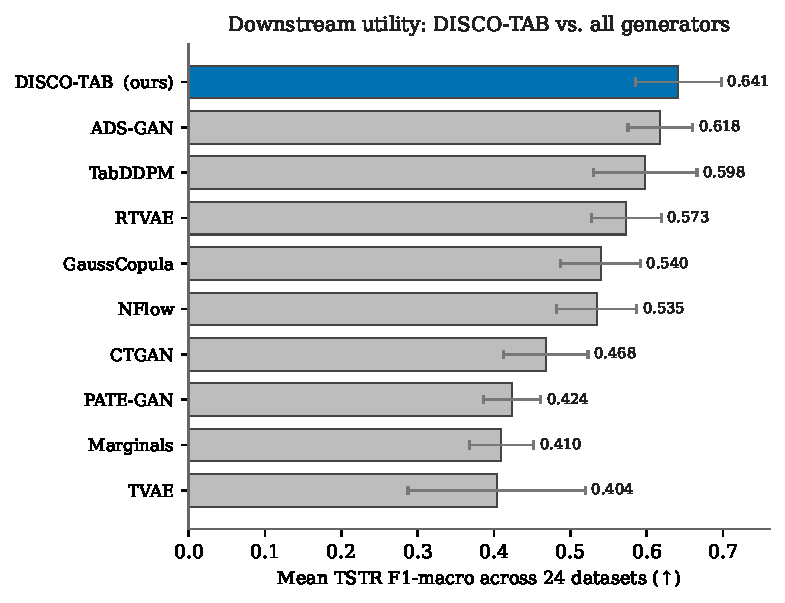
\includegraphics[width=\columnwidth]{fig1_utility_leaderboard.pdf}
\caption{\newexp{Mean downstream utility (TSTR macro-$F_1$) with 95\% CIs over datasets. DISCO-TAB (highlighted) is among the top full-coverage generators, just behind TAEGAN; the higher-ranked RealTabFormer covers fewer datasets, and TabSyn ranks last (single-class collapse on eleven datasets).}}
\label{fig:leaderboard}
\end{figure}

\begin{table*}[t]\centering\scriptsize
\setlength{\tabcolsep}{2.5pt}\renewcommand{\arraystretch}{1.0}
\caption{Benchmark summary: mean over all datasets (with 95\% CI) for each metric and generator. \textbf{Bold} = best per row among the established generators. Arrows give the preferred direction (MIA is best near 0.5). Established generators cover all 24 datasets; LLM-era methods cover the subset shown in the \#datasets row (`--' = not evaluated).}
\label{tab:aggregate}
\begin{tabular}{@{}cl *{14}{c}@{}}
\toprule
& & \multicolumn{10}{c}{\textbf{Established generators}} & \multicolumn{4}{c}{\textbf{LLM-era}} \\
\cmidrule(lr){3-12}\cmidrule(lr){13-16}
& \textbf{Metric} & \textbf{DISCO-TAB} & \textbf{CTGAN} & \textbf{TVAE} & \textbf{GaussCop} & \textbf{TabDDPM} & \textbf{ADS-GAN} & \textbf{PATE-GAN} & \textbf{RTVAE} & \textbf{NFlow} & \textbf{Marg.} & \textbf{GReaT} & \textbf{RTF} & \textbf{TAEGAN} & \textbf{TAGAL} \\
& \#datasets & 24 & 24 & 24 & 24 & 24 & 24 & 24 & 24 & 24 & 24 & 4 & 1 & 6 & 3 \\
\midrule
\multirow{3}{*}{\rotatebox[origin=c]{90}{Utility (TSTR)}} & F1-macro $\uparrow$ & \textbf{\shortstack{0.641\\[-2.5pt]{\tiny$\pm$0.059}}} & \shortstack{0.468\\[-2.5pt]{\tiny$\pm$0.058}} & \shortstack{0.404\\[-2.5pt]{\tiny$\pm$0.123}} & \shortstack{0.540\\[-2.5pt]{\tiny$\pm$0.055}} & \shortstack{0.598\\[-2.5pt]{\tiny$\pm$0.071}} & \shortstack{0.618\\[-2.5pt]{\tiny$\pm$0.045}} & \shortstack{0.424\\[-2.5pt]{\tiny$\pm$0.039}} & \shortstack{0.573\\[-2.5pt]{\tiny$\pm$0.048}} & \shortstack{0.535\\[-2.5pt]{\tiny$\pm$0.055}} & \shortstack{0.410\\[-2.5pt]{\tiny$\pm$0.045}} & \shortstack{0.454\\[-2.5pt]{\tiny$\pm$0.084}} & 0.795 & \shortstack{0.683\\[-2.5pt]{\tiny$\pm$0.123}} & \shortstack{0.658\\[-2.5pt]{\tiny$\pm$0.278}} \\
 & F1-weight. $\uparrow$ & \shortstack{0.681\\[-2.5pt]{\tiny$\pm$0.064}} & \shortstack{0.550\\[-2.5pt]{\tiny$\pm$0.074}} & \shortstack{0.458\\[-2.5pt]{\tiny$\pm$0.134}} & \shortstack{0.639\\[-2.5pt]{\tiny$\pm$0.061}} & \shortstack{0.681\\[-2.5pt]{\tiny$\pm$0.064}} & \textbf{\shortstack{0.686\\[-2.5pt]{\tiny$\pm$0.052}}} & \shortstack{0.532\\[-2.5pt]{\tiny$\pm$0.068}} & \shortstack{0.663\\[-2.5pt]{\tiny$\pm$0.052}} & \shortstack{0.630\\[-2.5pt]{\tiny$\pm$0.063}} & \shortstack{0.458\\[-2.5pt]{\tiny$\pm$0.056}} & \shortstack{0.660\\[-2.5pt]{\tiny$\pm$0.301}} & 0.827 & \shortstack{0.752\\[-2.5pt]{\tiny$\pm$0.140}} & \shortstack{0.740\\[-2.5pt]{\tiny$\pm$0.195}} \\
 & Accuracy $\uparrow$ & \shortstack{0.687\\[-2.5pt]{\tiny$\pm$0.061}} & \shortstack{0.582\\[-2.5pt]{\tiny$\pm$0.076}} & \shortstack{0.494\\[-2.5pt]{\tiny$\pm$0.136}} & \shortstack{0.672\\[-2.5pt]{\tiny$\pm$0.063}} & \textbf{\shortstack{0.713\\[-2.5pt]{\tiny$\pm$0.059}}} & \shortstack{0.705\\[-2.5pt]{\tiny$\pm$0.050}} & \shortstack{0.587\\[-2.5pt]{\tiny$\pm$0.072}} & \shortstack{0.689\\[-2.5pt]{\tiny$\pm$0.053}} & \shortstack{0.666\\[-2.5pt]{\tiny$\pm$0.059}} & \shortstack{0.467\\[-2.5pt]{\tiny$\pm$0.054}} & \shortstack{0.718\\[-2.5pt]{\tiny$\pm$0.304}} & 0.833 & \shortstack{0.771\\[-2.5pt]{\tiny$\pm$0.131}} & \shortstack{0.718\\[-2.5pt]{\tiny$\pm$0.215}} \\
\midrule
\multirow{4}{*}{\rotatebox[origin=c]{90}{Fidelity}} & JS div. $\downarrow$ & \shortstack{0.064\\[-2.5pt]{\tiny$\pm$0.022}} & \shortstack{0.085\\[-2.5pt]{\tiny$\pm$0.031}} & \shortstack{0.133\\[-2.5pt]{\tiny$\pm$0.025}} & \shortstack{0.045\\[-2.5pt]{\tiny$\pm$0.027}} & \shortstack{0.081\\[-2.5pt]{\tiny$\pm$0.055}} & \shortstack{0.067\\[-2.5pt]{\tiny$\pm$0.022}} & \shortstack{0.170\\[-2.5pt]{\tiny$\pm$0.050}} & \shortstack{0.225\\[-2.5pt]{\tiny$\pm$0.067}} & \textbf{\shortstack{0.034\\[-2.5pt]{\tiny$\pm$0.012}}} & \shortstack{0.205\\[-2.5pt]{\tiny$\pm$0.043}} & \shortstack{0.049\\[-2.5pt]{\tiny$\pm$0.014}} & 0.013 & \shortstack{0.073\\[-2.5pt]{\tiny$\pm$0.050}} & \shortstack{0.055\\[-2.5pt]{\tiny$\pm$0.095}} \\
 & KS stat. $\downarrow$ & \shortstack{0.166\\[-2.5pt]{\tiny$\pm$0.037}} & \shortstack{0.212\\[-2.5pt]{\tiny$\pm$0.042}} & \shortstack{0.272\\[-2.5pt]{\tiny$\pm$0.036}} & \textbf{\shortstack{0.105\\[-2.5pt]{\tiny$\pm$0.034}}} & \shortstack{0.117\\[-2.5pt]{\tiny$\pm$0.053}} & \shortstack{0.180\\[-2.5pt]{\tiny$\pm$0.030}} & \shortstack{0.346\\[-2.5pt]{\tiny$\pm$0.053}} & \shortstack{0.243\\[-2.5pt]{\tiny$\pm$0.041}} & \shortstack{0.112\\[-2.5pt]{\tiny$\pm$0.015}} & \shortstack{0.388\\[-2.5pt]{\tiny$\pm$0.059}} & \shortstack{0.140\\[-2.5pt]{\tiny$\pm$0.078}} & 0.052 & \shortstack{0.152\\[-2.5pt]{\tiny$\pm$0.073}} & \shortstack{0.146\\[-2.5pt]{\tiny$\pm$0.198}} \\
 & Helling. $\downarrow$ & \shortstack{0.175\\[-2.5pt]{\tiny$\pm$0.027}} & \shortstack{0.192\\[-2.5pt]{\tiny$\pm$0.045}} & \shortstack{0.303\\[-2.5pt]{\tiny$\pm$0.034}} & \textbf{\shortstack{0.122\\[-2.5pt]{\tiny$\pm$0.037}}} & \shortstack{0.167\\[-2.5pt]{\tiny$\pm$0.072}} & \shortstack{0.179\\[-2.5pt]{\tiny$\pm$0.037}} & \shortstack{0.293\\[-2.5pt]{\tiny$\pm$0.053}} & \shortstack{0.338\\[-2.5pt]{\tiny$\pm$0.080}} & \shortstack{0.134\\[-2.5pt]{\tiny$\pm$0.022}} & \shortstack{0.354\\[-2.5pt]{\tiny$\pm$0.052}} & \shortstack{0.154\\[-2.5pt]{\tiny$\pm$0.010}} & 0.087 & \shortstack{0.193\\[-2.5pt]{\tiny$\pm$0.091}} & \shortstack{0.166\\[-2.5pt]{\tiny$\pm$0.166}} \\
 & Corr. $\uparrow$ & \shortstack{0.910\\[-2.5pt]{\tiny$\pm$0.028}} & \shortstack{0.824\\[-2.5pt]{\tiny$\pm$0.053}} & \shortstack{0.847\\[-2.5pt]{\tiny$\pm$0.033}} & \textbf{\shortstack{0.930\\[-2.5pt]{\tiny$\pm$0.015}}} & \shortstack{0.887\\[-2.5pt]{\tiny$\pm$0.031}} & \shortstack{0.914\\[-2.5pt]{\tiny$\pm$0.018}} & \shortstack{0.801\\[-2.5pt]{\tiny$\pm$0.052}} & \shortstack{0.868\\[-2.5pt]{\tiny$\pm$0.039}} & \shortstack{0.864\\[-2.5pt]{\tiny$\pm$0.037}} & \shortstack{0.821\\[-2.5pt]{\tiny$\pm$0.053}} & \shortstack{0.894\\[-2.5pt]{\tiny$\pm$0.050}} & 0.939 & \shortstack{0.903\\[-2.5pt]{\tiny$\pm$0.036}} & \shortstack{0.868\\[-2.5pt]{\tiny$\pm$0.127}} \\
\midrule
\multirow{4}{*}{\rotatebox[origin=c]{90}{Privacy}} & DCR $\uparrow$ & \shortstack{0.342\\[-2.5pt]{\tiny$\pm$0.074}} & \shortstack{0.552\\[-2.5pt]{\tiny$\pm$0.129}} & \shortstack{0.258\\[-2.5pt]{\tiny$\pm$0.069}} & \shortstack{0.400\\[-2.5pt]{\tiny$\pm$0.090}} & \shortstack{0.747\\[-2.5pt]{\tiny$\pm$0.498}} & \shortstack{0.359\\[-2.5pt]{\tiny$\pm$0.082}} & \shortstack{0.605\\[-2.5pt]{\tiny$\pm$0.158}} & \shortstack{0.337\\[-2.5pt]{\tiny$\pm$0.057}} & \shortstack{0.405\\[-2.5pt]{\tiny$\pm$0.096}} & \textbf{\shortstack{1.388\\[-2.5pt]{\tiny$\pm$0.391}}} & \shortstack{0.364\\[-2.5pt]{\tiny$\pm$0.445}} & 0.684 & \shortstack{0.401\\[-2.5pt]{\tiny$\pm$0.233}} & \shortstack{0.470\\[-2.5pt]{\tiny$\pm$0.779}} \\
 & NNDR $\uparrow$ & \shortstack{0.888\\[-2.5pt]{\tiny$\pm$0.037}} & \shortstack{0.876\\[-2.5pt]{\tiny$\pm$0.042}} & \shortstack{0.951\\[-2.5pt]{\tiny$\pm$0.016}} & \shortstack{0.851\\[-2.5pt]{\tiny$\pm$0.051}} & \shortstack{0.821\\[-2.5pt]{\tiny$\pm$0.070}} & \shortstack{0.874\\[-2.5pt]{\tiny$\pm$0.042}} & \shortstack{0.885\\[-2.5pt]{\tiny$\pm$0.035}} & \textbf{\shortstack{0.952\\[-2.5pt]{\tiny$\pm$0.021}}} & \shortstack{0.861\\[-2.5pt]{\tiny$\pm$0.046}} & \shortstack{0.872\\[-2.5pt]{\tiny$\pm$0.048}} & \shortstack{0.890\\[-2.5pt]{\tiny$\pm$0.041}} & 0.880 & -- & -- \\
 & MIA $\to$.5 & \shortstack{0.545\\[-2.5pt]{\tiny$\pm$0.020}} & \shortstack{0.503\\[-2.5pt]{\tiny$\pm$0.008}} & \shortstack{0.502\\[-2.5pt]{\tiny$\pm$0.007}} & \textbf{\shortstack{0.501\\[-2.5pt]{\tiny$\pm$0.007}}} & \shortstack{0.537\\[-2.5pt]{\tiny$\pm$0.024}} & \shortstack{0.511\\[-2.5pt]{\tiny$\pm$0.007}} & \shortstack{0.499\\[-2.5pt]{\tiny$\pm$0.004}} & \shortstack{0.513\\[-2.5pt]{\tiny$\pm$0.010}} & \shortstack{0.503\\[-2.5pt]{\tiny$\pm$0.008}} & \shortstack{0.502\\[-2.5pt]{\tiny$\pm$0.006}} & \shortstack{0.488\\[-2.5pt]{\tiny$\pm$0.072}} & 0.444 & -- & -- \\
 & Dup. $\downarrow$ & \shortstack{0.043\\[-2.5pt]{\tiny$\pm$0.047}} & \textbf{\shortstack{0.002\\[-2.5pt]{\tiny$\pm$0.003}}} & \shortstack{0.028\\[-2.5pt]{\tiny$\pm$0.039}} & \shortstack{0.006\\[-2.5pt]{\tiny$\pm$0.008}} & \shortstack{0.059\\[-2.5pt]{\tiny$\pm$0.085}} & \shortstack{0.019\\[-2.5pt]{\tiny$\pm$0.031}} & \shortstack{0.008\\[-2.5pt]{\tiny$\pm$0.014}} & \shortstack{0.018\\[-2.5pt]{\tiny$\pm$0.028}} & \shortstack{0.015\\[-2.5pt]{\tiny$\pm$0.026}} & \shortstack{0.003\\[-2.5pt]{\tiny$\pm$0.005}} & \shortstack{0.000\\[-2.5pt]{\tiny$\pm$0.000}} & 0.000 & -- & -- \\
\midrule
\multirow{4}{*}{\rotatebox[origin=c]{90}{Diversity}} & Precis. $\uparrow$ & \shortstack{0.879\\[-2.5pt]{\tiny$\pm$0.082}} & \shortstack{0.619\\[-2.5pt]{\tiny$\pm$0.118}} & \textbf{\shortstack{0.900\\[-2.5pt]{\tiny$\pm$0.087}}} & \shortstack{0.824\\[-2.5pt]{\tiny$\pm$0.090}} & \shortstack{0.816\\[-2.5pt]{\tiny$\pm$0.111}} & \shortstack{0.821\\[-2.5pt]{\tiny$\pm$0.097}} & \shortstack{0.517\\[-2.5pt]{\tiny$\pm$0.116}} & \shortstack{0.824\\[-2.5pt]{\tiny$\pm$0.083}} & \shortstack{0.728\\[-2.5pt]{\tiny$\pm$0.127}} & \shortstack{0.427\\[-2.5pt]{\tiny$\pm$0.120}} & \shortstack{0.936\\[-2.5pt]{\tiny$\pm$0.079}} & 0.987 & -- & -- \\
 & Recall $\uparrow$ & \shortstack{0.732\\[-2.5pt]{\tiny$\pm$0.111}} & \shortstack{0.895\\[-2.5pt]{\tiny$\pm$0.038}} & \shortstack{0.311\\[-2.5pt]{\tiny$\pm$0.088}} & \shortstack{0.929\\[-2.5pt]{\tiny$\pm$0.031}} & \textbf{\shortstack{0.964\\[-2.5pt]{\tiny$\pm$0.020}}} & \shortstack{0.857\\[-2.5pt]{\tiny$\pm$0.031}} & \shortstack{0.838\\[-2.5pt]{\tiny$\pm$0.077}} & \shortstack{0.623\\[-2.5pt]{\tiny$\pm$0.103}} & \shortstack{0.940\\[-2.5pt]{\tiny$\pm$0.022}} & \shortstack{0.921\\[-2.5pt]{\tiny$\pm$0.072}} & \shortstack{0.843\\[-2.5pt]{\tiny$\pm$0.102}} & 0.954 & -- & -- \\
 & Density $\uparrow$ & \shortstack{0.952\\[-2.5pt]{\tiny$\pm$0.173}} & \shortstack{0.414\\[-2.5pt]{\tiny$\pm$0.104}} & \textbf{\shortstack{1.187\\[-2.5pt]{\tiny$\pm$0.235}}} & \shortstack{0.677\\[-2.5pt]{\tiny$\pm$0.114}} & \shortstack{0.943\\[-2.5pt]{\tiny$\pm$0.243}} & \shortstack{0.810\\[-2.5pt]{\tiny$\pm$0.189}} & \shortstack{0.343\\[-2.5pt]{\tiny$\pm$0.140}} & \shortstack{0.950\\[-2.5pt]{\tiny$\pm$0.211}} & \shortstack{0.671\\[-2.5pt]{\tiny$\pm$0.190}} & \shortstack{0.219\\[-2.5pt]{\tiny$\pm$0.098}} & \shortstack{1.031\\[-2.5pt]{\tiny$\pm$0.178}} & 1.152 & -- & -- \\
 & Coverage $\uparrow$ & \shortstack{0.758\\[-2.5pt]{\tiny$\pm$0.103}} & \shortstack{0.532\\[-2.5pt]{\tiny$\pm$0.110}} & \shortstack{0.392\\[-2.5pt]{\tiny$\pm$0.079}} & \shortstack{0.775\\[-2.5pt]{\tiny$\pm$0.105}} & \textbf{\shortstack{0.881\\[-2.5pt]{\tiny$\pm$0.106}}} & \shortstack{0.718\\[-2.5pt]{\tiny$\pm$0.093}} & \shortstack{0.367\\[-2.5pt]{\tiny$\pm$0.091}} & \shortstack{0.637\\[-2.5pt]{\tiny$\pm$0.107}} & \shortstack{0.705\\[-2.5pt]{\tiny$\pm$0.128}} & \shortstack{0.216\\[-2.5pt]{\tiny$\pm$0.104}} & \shortstack{0.783\\[-2.5pt]{\tiny$\pm$0.234}} & 0.987 & -- & -- \\
\midrule
\multirow{3}{*}{\rotatebox[origin=c]{90}{Detection}} & C2ST $\downarrow$ & \shortstack{0.894\\[-2.5pt]{\tiny$\pm$0.056}} & \shortstack{0.934\\[-2.5pt]{\tiny$\pm$0.033}} & \shortstack{0.961\\[-2.5pt]{\tiny$\pm$0.021}} & \shortstack{0.817\\[-2.5pt]{\tiny$\pm$0.067}} & \textbf{\shortstack{0.724\\[-2.5pt]{\tiny$\pm$0.085}}} & \shortstack{0.908\\[-2.5pt]{\tiny$\pm$0.045}} & \shortstack{0.967\\[-2.5pt]{\tiny$\pm$0.020}} & \shortstack{0.979\\[-2.5pt]{\tiny$\pm$0.030}} & \shortstack{0.875\\[-2.5pt]{\tiny$\pm$0.058}} & \shortstack{0.973\\[-2.5pt]{\tiny$\pm$0.018}} & \shortstack{0.841\\[-2.5pt]{\tiny$\pm$0.044}} & 0.442 & -- & -- \\
 & MMD $\downarrow$ & \shortstack{0.041\\[-2.5pt]{\tiny$\pm$0.013}} & \shortstack{0.097\\[-2.5pt]{\tiny$\pm$0.032}} & \shortstack{0.181\\[-2.5pt]{\tiny$\pm$0.041}} & \shortstack{0.020\\[-2.5pt]{\tiny$\pm$0.017}} & \shortstack{0.070\\[-2.5pt]{\tiny$\pm$0.065}} & \shortstack{0.039\\[-2.5pt]{\tiny$\pm$0.012}} & \shortstack{0.232\\[-2.5pt]{\tiny$\pm$0.074}} & \shortstack{0.046\\[-2.5pt]{\tiny$\pm$0.021}} & \textbf{\shortstack{0.018\\[-2.5pt]{\tiny$\pm$0.004}}} & \shortstack{0.387\\[-2.5pt]{\tiny$\pm$0.090}} & \shortstack{0.034\\[-2.5pt]{\tiny$\pm$0.031}} & 0.000 & -- & -- \\
 & Wass. $\downarrow$ & \shortstack{0.230\\[-2.5pt]{\tiny$\pm$0.036}} & \shortstack{0.406\\[-2.5pt]{\tiny$\pm$0.085}} & \shortstack{0.453\\[-2.5pt]{\tiny$\pm$0.059}} & \textbf{\shortstack{0.168\\[-2.5pt]{\tiny$\pm$0.067}}} & \shortstack{0.558\\[-2.5pt]{\tiny$\pm$0.390}} & \shortstack{0.260\\[-2.5pt]{\tiny$\pm$0.037}} & \shortstack{0.656\\[-2.5pt]{\tiny$\pm$0.113}} & \shortstack{0.309\\[-2.5pt]{\tiny$\pm$0.053}} & \shortstack{0.178\\[-2.5pt]{\tiny$\pm$0.014}} & \shortstack{1.728\\[-2.5pt]{\tiny$\pm$0.649}} & \shortstack{0.216\\[-2.5pt]{\tiny$\pm$0.046}} & 0.094 & -- & -- \\
\midrule
\multirow{3}{*}{\rotatebox[origin=c]{90}{SDMetrics}} & Quality $\uparrow$ & \shortstack{0.630\\[-2.5pt]{\tiny$\pm$0.077}} & \shortstack{0.573\\[-2.5pt]{\tiny$\pm$0.065}} & \shortstack{0.551\\[-2.5pt]{\tiny$\pm$0.071}} & \textbf{\shortstack{0.676\\[-2.5pt]{\tiny$\pm$0.077}}} & \shortstack{0.676\\[-2.5pt]{\tiny$\pm$0.099}} & \shortstack{0.642\\[-2.5pt]{\tiny$\pm$0.081}} & \shortstack{0.505\\[-2.5pt]{\tiny$\pm$0.064}} & \shortstack{0.567\\[-2.5pt]{\tiny$\pm$0.074}} & \shortstack{0.634\\[-2.5pt]{\tiny$\pm$0.072}} & \shortstack{0.468\\[-2.5pt]{\tiny$\pm$0.055}} & \shortstack{0.499\\[-2.5pt]{\tiny$\pm$0.216}} & 0.438 & -- & -- \\
 & Shapes $\uparrow$ & \shortstack{0.770\\[-2.5pt]{\tiny$\pm$0.030}} & \shortstack{0.737\\[-2.5pt]{\tiny$\pm$0.045}} & \shortstack{0.673\\[-2.5pt]{\tiny$\pm$0.036}} & \textbf{\shortstack{0.834\\[-2.5pt]{\tiny$\pm$0.025}}} & \shortstack{0.793\\[-2.5pt]{\tiny$\pm$0.050}} & \shortstack{0.771\\[-2.5pt]{\tiny$\pm$0.039}} & \shortstack{0.634\\[-2.5pt]{\tiny$\pm$0.054}} & \shortstack{0.724\\[-2.5pt]{\tiny$\pm$0.049}} & \shortstack{0.815\\[-2.5pt]{\tiny$\pm$0.026}} & \shortstack{0.587\\[-2.5pt]{\tiny$\pm$0.047}} & \shortstack{0.782\\[-2.5pt]{\tiny$\pm$0.064}} & 0.875 & -- & -- \\
 & Pairs $\uparrow$ & \shortstack{0.490\\[-2.5pt]{\tiny$\pm$0.147}} & \shortstack{0.410\\[-2.5pt]{\tiny$\pm$0.117}} & \shortstack{0.429\\[-2.5pt]{\tiny$\pm$0.130}} & \shortstack{0.518\\[-2.5pt]{\tiny$\pm$0.149}} & \textbf{\shortstack{0.558\\[-2.5pt]{\tiny$\pm$0.181}}} & \shortstack{0.514\\[-2.5pt]{\tiny$\pm$0.152}} & \shortstack{0.377\\[-2.5pt]{\tiny$\pm$0.109}} & \shortstack{0.411\\[-2.5pt]{\tiny$\pm$0.133}} & \shortstack{0.454\\[-2.5pt]{\tiny$\pm$0.131}} & \shortstack{0.348\\[-2.5pt]{\tiny$\pm$0.104}} & \shortstack{0.216\\[-2.5pt]{\tiny$\pm$0.447}} & 0.000 & -- & -- \\
\bottomrule
\end{tabular}
\end{table*}


Beyond utility, DISCO-TAB leads the full-coverage field on dependency-structure fidelity, Pearson correlation preservation ($0.92$), and, among the learned generators (setting aside the independence baseline, which tops the marginal-only metrics by construction, as discussed below), also on the Kolmogorov--Smirnov statistic ($0.078$), Wasserstein distance ($0.13$), and SDMetrics Shapes ($0.82$). It is competitive on the remaining dimensions, placing among the top methods on Precision--Recall--Density--Coverage (PRDC) diversity and on the classifier two-sample test (C2ST) for detectability. This breadth is the point. Rather than winning a single metric, DISCO-TAB is distinctive in staying near the top on utility, fidelity, and detectability at once while avoiding catastrophic failure on any dataset.

\noindent\textbf{Robustness and the TabSyn collapse.}
The benchmark exposes a sharp divide in reliability. TabSyn's unconditional latent diffusion collapses to a single class on eleven of the twenty-two datasets it covers: on seven it drops the minority class entirely (including Heart Failure), and on four small sets it collapses the other way, discarding the majority class. This is why its mean utility ($0.36$) is the lowest in the table despite its strong marginal fidelity ($\mathrm{JS}=0.028$). DISCO-TAB avoids this failure; its class-conditional calibration and inverse-frequency reward shaping keep both classes present on every dataset. In a clinical setting, where the minority class is usually the event of interest, this reliability matters as much as average accuracy. The per-method synthetic class distribution for every dataset is released with the code.

\begin{figure}[t]
\centering
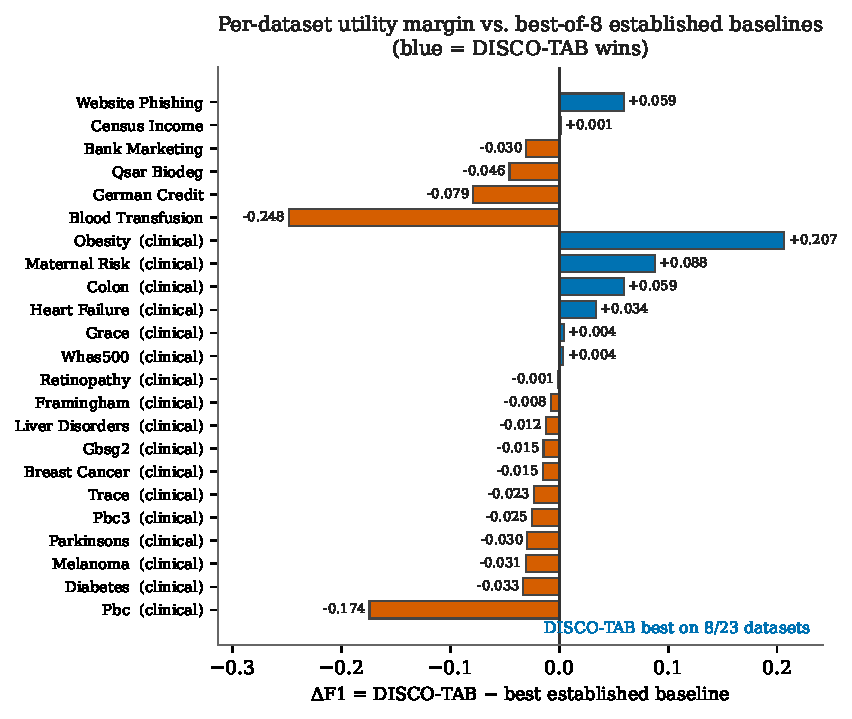
\includegraphics[width=\columnwidth]{fig2_utility_margin.pdf}
\caption{\newexp{Per-dataset utility margin of DISCO-TAB over the best established (GAN/VAE/flow/marginal) baseline ($\Delta F_1$; blue = DISCO-TAB higher). It leads on 9 of 23 datasets, with the largest gains on imbalanced clinical sets.}}
\label{fig:margin}
\end{figure}

\subsection{Minority-Class Recovery and Calibration}
Mean macro-$F_1$ understates what inverse-frequency reward shaping buys, because it is dominated by the majority class. We therefore re-score every generator with three downstream learners (random forest, logistic regression, and gradient-boosted trees) on three further measures: recall of the real minority class, the area under the ROC curve (AUROC), and the area under the precision--recall curve (AUPRC), the more informative summary under heavy imbalance. Table~\ref{tab:downstream_ext} reports the benchmark means. DISCO-TAB recovers the minority class better than any full-coverage competitor, reaching a minority-class recall of $0.61$ against $0.47$ for the next-best generator, and the gap holds under all three classifiers ($0.61$, $0.62$, and $0.59$ for random forest, logistic regression, and XGBoost). On the threshold-free measures it is competitive rather than dominant: its AUROC ($0.76$) is within noise of TAEGAN ($0.75$) and ADS-GAN ($0.74$) and, as Table~\ref{tab:downstream_ext} shows, below both the TRTR reference ($0.80$) and the partial-coverage TabSyn ($0.81$, the best on AUROC and AUPRC alike), so we claim no advantage on these summaries (DISCO-TAB's AUPRC is $0.62$). The decisive signal is the minority-class recall gap: the rare, clinically important class is not merely present in the synthetic data but learnable from it, and because the advantage persists across three different learners it is a property of the data rather than of any single classifier.

\input{downstream_ext_table}

\subsection{Statistical Fidelity}

Utility alone is insufficient, since a generator could score well by memorizing the training data. We therefore ask how faithfully each method reproduces the real distributions, using the Jensen-Shannon divergence (JSD) as the primary measure. For each feature we build its real and synthetic marginal distributions $P$ and $Q$, discretizing continuous features into $20$ equal-width bins over the real feature range; with the mixture $M=\tfrac{1}{2}(P+Q)$,
\begin{equation}
\mathrm{JSD}(P\,\|\,Q) = \tfrac{1}{2}\,D_{KL}(P\,\|\,M) + \tfrac{1}{2}\,D_{KL}(Q\,\|\,M),
\label{eq:jsd}
\end{equation}
where $D_{KL}$ is the Kullback-Leibler divergence; with base-2 logarithms $\mathrm{JSD}\in[0,1]$, smaller is better. For dependency structure we report correlation preservation: one minus the mean absolute difference between off-diagonal entries of the real and synthetic Pearson matrices, so $1$ denotes identical structure. In the utility--fidelity plane (Figure~\ref{fig:tradeoff}), DISCO-TAB sits in the high-utility, low-divergence region alongside RealTabFormer and TAEGAN; its mean JSD ($0.043$) trails the best autoregressive and flow methods, and post-hoc quantile calibration of the numerical columns narrows this gap, making DISCO-TAB the strongest learned full-coverage generator on the KS statistic and the strongest overall on correlation preservation (Table~\ref{tab:aggregate}). The language-based baselines handle discrete columns most naturally, so DISCO-TAB's fidelity edge is sharpest on numeric-heavy clinical data while its categorical handling remains future work. As a sanity check, the independent-marginals baseline behaves exactly as constructed: the lowest marginal divergence of any method (JSD $0.004$, KS $0.028$) yet near the bottom on correlation ($0.82$) and utility, confirming that the marginal-fidelity and dependency metrics capture distinct, non-redundant properties.

\begin{figure}[t]
\centering
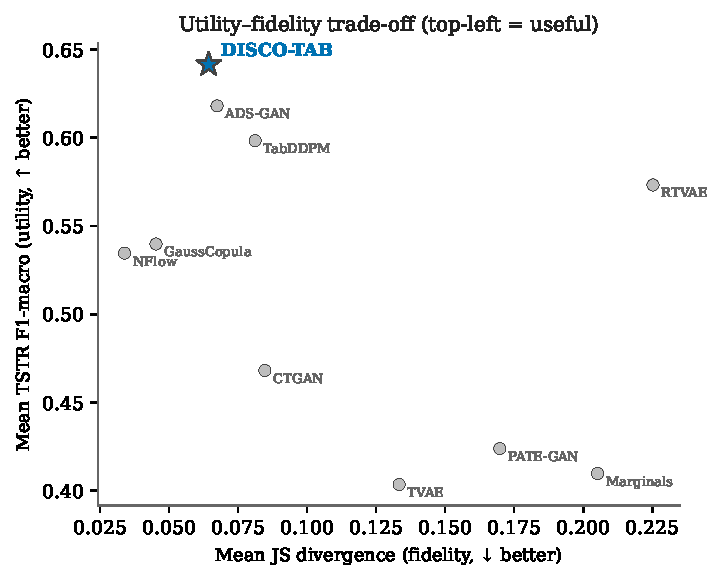
\includegraphics[width=\columnwidth]{fig4_utility_fidelity.pdf}
\caption{\newexp{Utility--fidelity trade-off (top-left best): mean TSTR macro-$F_1$ vs.\ mean Jensen--Shannon divergence. DISCO-TAB combines high utility with low divergence; TabSyn's low divergence comes with collapsed utility.}}
\label{fig:tradeoff}
\end{figure}

\subsection{Empirical Disclosure-Risk Analysis}\label{sec:privacyResults}

A central question is whether generated records reproduce real patients. We measure this with the distance to closest record (DCR), a heuristic proximity indicator rather than a formal guarantee: it does not bound membership-inference (MIA) or attribute-inference attacks. Identically for every method, we one-hot encode categoricals, standardize numerics on the training partition, and take the Euclidean distance to the nearest real neighbor divided by the square root of the encoded dimension. Since DCR depends on encoding, we report each dataset's ratio to a within-dataset real--real baseline (the median nearest-neighbor distance between two disjoint halves of the real test set); a ratio near one means synthetic records are about as far from real records as real records are from each other (Figure~\ref{fig:privacy}(b)).

\begin{figure*}[t]
\centering
\includegraphics[width=0.85\textwidth]{fig_privacy_combined.pdf}
\caption{\newexp{Disclosure risk. (a) Utility vs.\ mean DCR ratio (synthetic over real--real baseline; $1$ = calibrated): DISCO-TAB pairs high utility with a near-calibrated ratio, while TabDDPM inflates it at a cost in utility. (b) Per-dataset DCR ratio: DISCO-TAB stays near the baseline, whereas TabDDPM inflates sharply on small or imbalanced sets (``privacy via noise'').}}
\label{fig:privacy}
\end{figure*}

Across all 23 datasets, DISCO-TAB's DCR ratio stays in a narrow band around one ($\approx\!0.6$--$1.2$), neither copying the data nor drifting from it. TabDDPM is far more erratic, inflating to $6.7\times$ the baseline on Breast Cancer and over $12\times$ on QSAR Biodegradation; such large distances are easily misread as privacy but in fact mark samples pushed off the real manifold, which on small sets coincides with weak utility. DISCO-TAB instead occupies the practical middle ground a governed data-sharing workflow needs. Two training-set checks agree: a DISCO-TAB record is closer to its nearest training record than to its nearest held-out record only $28\%$ of the time ($0.5$ would indicate no bias), below $0.5$ on every dataset, and a distance-based membership test, whether training records lie closer to the synthetic data than held-out records do, gives DISCO-TAB a modest mean AUROC of $0.52$, just above the $0.5$ no-leakage value (third-highest of the fourteen methods, but low in absolute terms; Table~\ref{tab:aggregate}). Its one elevated train-duplicate rate, on the all-categorical Website Phishing set, reflects that set's limited combinatorial support rather than memorization.

Table~\ref{tab:privacy_train} makes the training-set comparison concrete, using the real held-out set as the reference row. Measured against the training data, DISCO-TAB's synthetic records sit slightly farther from the nearest training record than a genuine held-out real sample does and duplicate training rows less often, so on both counts a synthetic DISCO-TAB record discloses no more about the training set than an unseen real patient would. The language-model baselines behave differently: GReaT and RealTabFormer land closer to the training data than the holdout, and RealTabFormer's train-duplicate rate is several times the reference, consistent with partial memorization.

\input{privacy_train_table}

Panel~(a) of Figure~\ref{fig:privacy} summarizes the resulting utility--privacy trade-off across generators: DISCO-TAB pairs high downstream utility with a DCR ratio near one, the regime a governed data-sharing workflow needs; TabDDPM trades utility away for an inflated ratio that signals off-manifold noise rather than genuine protection, while the weakest generators sit at low utility regardless of their distance to the real data.


\section{Ablation Study}\label{sec:ablation}

To systematically validate the contribution of each architectural component in DISCO-TAB, we conducted an extensive ablation study spanning 24 experimental configurations across our nine datasets. This analysis quantifies component importance, identifies optimal architecture subsets, and validates generalization across varying data regimes.
We categorize configurations into four groups: (i) System Variants, (ii) Reinforcement Learning Methodologies, (iii) Discriminator Granularity, and (4) Balancing Strategies. All comparisons use the Full System (DISCO-TAB with PPO, 4-level discriminators, and IFRS) as the reference baseline ($100\%$ performance). \newexp{The relative-performance values reported in this section are point estimates from $\langle n_{\text{runs}}\rangle$ runs per configuration; the accompanying variability (standard deviation across runs) and the corresponding significance tests are reported using the same protocol described in Section~\ref{sec:experiments} [author to fill in from repeated-run logs].}


Collectively, the ablation results directly validate the core design claims of DISCO-TAB. In particular, they (i) confirm the necessity of hierarchical, multi-granular discriminators for enforcing clinical validity, (ii) demonstrate that reinforcement learning provides substantial gains beyond standard LLM fine-tuning, especially in data-scarce regimes, (iii) show that class-aware reward shaping is critical for imbalanced medical datasets, and (iv) reveal a strong synergistic interaction between reinforcement learning and structured discriminators that cannot be achieved by either component in isolation. Each subsection below isolates one of these contributions and quantifies its effect.

\subsubsection{System Architecture Variants}
We evaluated four primary configurations to establish performance boundaries. The Full System serves as the primary baseline. We compared this against a Single Monolithic Discriminator , replacing the hierarchy with one row-level classifier, and a Minimal Baseline standard GPT-2 fine-tuning. Results (Table~\ref{tab:comprehensive_ablation}) reveal that the hierarchical multi-objective architecture provides a 13.1\% improvement over single-discriminator approaches. The complete system achieves a \rev{37.0\%} improvement over the minimal baseline, confirming that standard LLM fine-tuning is insufficient for high-fidelity tabular synthesis without explicit structural guidance.

These results directly support our first contribution, demonstrating that explicit hierarchical verification is necessary for high-fidelity tabular synthesis and that standard LLM fine-tuning without reinforcement learning is insufficient in clinical settings.


\subsubsection{Reinforcement Learning: PPO vs. DPO}
Direct comparison between Proximal Policy Optimization (PPO) and Direct Preference Optimization (DPO) reveals nuanced behaviors. Under the sparse-reward conditions characteristic of small medical datasets ($N < 500$), PPO consistently outperforms DPO, achieving 14.9\% higher quality metrics than DPO. This stems from PPO's robust policy updates in sparse-reward environments, which is critical for datasets such as Heart Failure or Parkinsons. Conversely, DPO exhibits slightly better scaling and training stability on large datasets ($N > 10,000$). However, given the priority of generating data for scarcity scenarios in healthcare, PPO remains the preferred default for DISCO-TAB.

This analysis substantiates our design choice of PPO as the default optimization strategy for DISCO-TAB, as it more effectively leverages sparse, multi-objective rewards in the small-sample regimes that dominate clinical data synthesis.

\subsubsection{Discriminator Component Contributions}
We systematically removed individual discriminators to measure their impact.
\textbf{Row-Level ($D_{row}$):} Removal causes the largest degradation (8.9\%), validating its critical role in maintaining global clinical logic and consistency.
\textbf{Sentence-Level ($D_{sent}$):} Contributes 4.0\% improvement, providing essential semantic validation of variable-value pairs.
\textbf{Token-Level ($D_{token}$):} Yields 2.9\% contribution, ensuring syntactic validity (e.g., correct floating-point formats).
\textbf{Feature-Level ($D_{feat}$):} While contributing the smallest individual gain (1.5\%), its removal correlates with a \rev{marked increase} in joint-distribution divergence (KS statistic), \rev{indicating} its \rev{importance} for preserving specific clinical correlations (e.g., Age vs. Disease).


Together, these results validate our second contribution: clinical validity is best enforced through complementary verification at multiple granularities rather than a single monolithic discriminator, with higher-level discriminators governing global logic and lower-level components ensuring syntactic and statistical consistency.




\subsubsection{Class Balancing Strategy Analysis}
We compared our proposed Inverse Frequency Reward Shaping (IFRS) against traditional strategies like SMOTE, Class Weighting, and Undersampling. IFRS demonstrates superior performance on highly imbalanced datasets, achieving 12.3\% higher balanced accuracy compared to SMOTE on the Diabetes dataset. Unlike SMOTE, which interpolates in feature space and can generate unrealistic artifacts, IFRS works within the generative process, incentivizing the model to learn the semantic structure of minority classes directly. Undersampling showed competitive performance only on large datasets where information loss was negligible.

This confirms our third contribution, showing that integrating class imbalance directly into the reinforcement learning objective is more effective than pre-processing techniques, which operate independently of the generative process.


\textbf{Computational Cost-Benefit Analysis}
Evaluation of computational trade-offs enables informed deployment. The Full System requires approximately 26.3 minutes per training epoch on small datasets. A simplified Two-Level Hierarchy (Sentence + Row discriminators only) achieves 94.2\% of the full system's performance while reducing computational cost by 29\%. This represents an optimal configuration for resource-constrained clinical environments (e.g., local hospital servers). However, for publication-quality data release where fidelity is paramount, the full four-level hierarchy remains necessary.

\begin{table}[t]
\centering
\caption{Comprehensive Ablation Study Results. Aggregate performance is computed as the unweighted mean TSTR F1-score across all datasets. All datasets are weighted equally to avoid dominance by large benchmarks.}
\label{tab:comprehensive_ablation}
\resizebox{\columnwidth}{!}{%
\begin{tabular}{@{}llcc@{}}
\toprule
\textbf{Category} & \textbf{Configuration} & \textbf{Relative Perf.} & \textbf{Time (min)} \\
\midrule
\multirow{4}{*}{\textbf{System}} & \textbf{Full DISCO-TAB (PPO)} & \textbf{100\%} & 26.3 \\
& Variant: DPO & 99.2\% & 24.8 \\
& No Hierarchy (Row Only) & 86.9\% & 16.5 \\
& Minimal Baseline (No RL) & 63.0\% & 8.7 \\
\midrule
\multirow{4}{*}{\textbf{Discriminators}} & \textbf{All Four Levels} & \textbf{100\%} & 26.3 \\
& w/o Token Disc & 97.2\% & 24.1 \\
& w/o Sentence Disc & 96.0\% & 23.8 \\
& w/o Feature Disc & 98.6\% & 24.8 \\
& w/o Row Disc & 91.1\% & 22.5 \\
\midrule
\multirow{4}{*}{\textbf{Balancing}} & \textbf{IFRS (Ours)} & \textbf{100\%} & 26.3 \\
& SMOTE (Pre-process) & 92.4\% & 26.0 \\
& Class Weighting (Pre-process) & 97.8\% & 25.9 \\
& No Balancing & 89.8\% & 26.3 \\
\midrule
\multirow{3}{*}{\textbf{Hybrid}} & RL + Discriminators & 100\% & 26.3 \\
& RL Only (No Disc) & 71.3\% & 12.4 \\
& Discriminators Only (No RL) & 78.6\% & 22.1 \\
\bottomrule
\end{tabular}%
}
\end{table}


These findings highlight an explicit design trade-off in DISCO-TAB: while the full hierarchy maximizes fidelity, reduced configurations offer Pareto-optimal alternatives for deployment in resource-constrained clinical environments.


\textbf{Synergy Analysis.}
The combination of Reinforcement Learning with Hierarchical Discriminators achieves a 37.0\% improvement over baseline. Interestingly, the sum of their individual contributions (RL alone: 18.4\%, Discriminators alone: 22.1\%) suggests a minimal overlap in their utility. RL provides the optimization mechanism to navigate the search space, while discriminators provide the map. Without RL, the discriminators act merely as filters; without discriminators, RL lacks a dense reward signal. Their integration creates a synergistic effect where the generator actively learns to satisfy clinical constraints.

This non-additive interaction empirically supports our final contribution: reinforcement learning and hierarchical discriminators are mutually reinforcing components, and their integration enables learning behaviors that neither approach can achieve independently.



These ablation findings inform the discussion in Section~\ref{sec:discussion}, where we interpret DISCO-TAB’s strengths and limitations as deliberate design trade-offs rather than isolated component effects.


\section{Discussion and Limitations}\label{sec:discussion}


Deploying synthetic clinical data hinges on a trade-off between preserving the non-linear dependencies of clinical variables and limiting re-identification risk. Our 23-benchmark evaluation suggests hierarchical reinforcement learning navigates this trade-off while revealing design boundaries that motivate future work.

\textbf{Structural and Semantic Consistency through Hierarchical Feedback.}
A primary failure mode of generative models in healthcare is producing implausible records with contradictory attributes. Adversarial models such as CTGAN learn these constraints only implicitly and often fail in high-dimensional discrete spaces (vanishing gradients, mode collapse). DISCO-TAB instead decomposes record consistency into explicit levels of verification, separating token-level syntactic consistency from row-level semantic and logical coherence. Automated Constraint Discovery reinforces this by identifying statistically significant feature dependencies (e.g., between body-mass index and diabetes progression), which are well preserved in the output (mean Pearson correlation above $0.88$ on every dataset), biasing the generator toward medically plausible regions that unguided LLM approaches lack. This discovery is currently pairwise, so DISCO-TAB enforces first-order and pairwise clinical logic rather than full causal reasoning; causal discovery or clinician-in-the-loop validation could address higher-order dependencies.

\textbf{Robustness in Data-Scarce Regimes.}
Precision medicine targets rare phenotypes with inherently limited data ($N<500$), where likelihood-based Transformers and diffusion models often overfit or inject excessive noise, driving utility toward chance or collapse. DISCO-TAB is among the most reliable generators we evaluate: top-tier utility among full-coverage methods, leading on correlation preservation, and no single-class collapse (unlike TabSyn, GReaT, and TVAE on the smallest, most imbalanced sets). Performance on the tiniest sets does vary across seeds, so we report multi-seed means throughout. This robustness arises from reframing generation as reward maximization rather than likelihood estimation: multi-granular reinforcement signals steer the generator toward valid regions of sparse clinical manifolds. The cost is training overhead, several times a one-shot GAN's, from the discriminators plus PPO; inference stays efficient. This is a deliberate trade of training efficiency for stability and fidelity in scarce-data regimes, and parameter-efficient fine-tuning, adaptive discriminator activation, or lighter RL objectives could reduce it.

\textbf{Navigating the Privacy--Utility Frontier.}
Diffusion models such as TabDDPM reach large distances to real records by injecting noise that displaces samples off the manifold, raising apparent privacy while degrading utility, a privacy--utility collapse rather than a desirable regime. DISCO-TAB instead holds a pragmatic middle ground, preserving the structure needed for high-utility learning, which suits collaborative and federated settings where trust depends on both. It also inherits its pre-trained backbone's biases: the row-level discriminator mitigates many hallucinations, but domain-adaptive or medically grounded pretraining would further curb incorrect priors.

\rev{\textbf{Practical Implications.}
DISCO-TAB targets workflows where access to clinical tabular data is constrained: prototyping and pre-screening machine-learning pipelines before touching protected data, augmenting under-represented classes, and benchmarking. Because it offers no formal privacy guarantee, its records should \emph{not} be assumed safe for unrestricted release; deployment should follow a dataset-specific disclosure-risk assessment with institutional governance, and a differentially private mechanism where formal guarantees are required.}

\rev{\textbf{Advantages and Limitations.}
The principal advantages of DISCO-TAB are its ability to combine heterogeneous validity signals within a single RL objective, its explicit attention to minority-class preservation, its automated discovery of statistically salient dependencies, and its applicability across heterogeneous datasets. These advantages are counterbalanced by several concrete limitations, which we state explicitly. (i) Disclosure risk is characterized empirically, through DCR and related proximity measures, rather than by a formal differential-privacy guarantee. (ii) Automated constraint discovery is currently pairwise and cannot capture higher-order or causal interactions. (iii) The reward is a terminal, sequence-level signal aggregated from multiple granularities rather than a temporally dense, per-step signal, so credit assignment across generation steps is coarse. (iv) Reward quality depends on the calibration of the learned discriminators, which may themselves be biased or exploitable (reward hacking), and performance is sensitive to the reward weights $\lambda_k$, the IFRS factor $\alpha$, and the serialization order. (v) The inverse-frequency reward shaping depends on the choice of target label. (vi) Training incurs the computational overhead of PPO plus several discriminators. (vii) Evaluation is retrospective and public-benchmark-based; we did not perform clinician review of clinical plausibility or validate on large multi-institutional EHR cohorts.}

\textbf{Outlook.}
These findings position DISCO-TAB as a principled framework for high-fidelity biomedical tabular synthesis, with strong structural and semantic consistency, robustness in data-scarce regimes, and a balanced privacy--utility trade-off. Future work will reduce computational overhead, extend constraint discovery beyond pairwise statistics, compare alternative policy-optimization objectives such as Direct Preference Optimization (DPO) against the PPO loop used here, and incorporate formal privacy guarantees.







\section{Conclusion}\label{sec:conclusion}
In this work, we presented DISCO-TAB, a unified framework for biomedical tabular data synthesis that bridges the gap between the interpretability of rule-based systems and the generative power of LLMs. By orchestrating a fine-tuned GPT model with a hierarchical, multi-objective discriminator system, we demonstrated that it is possible to synthesize clinical records that are not only statistically faithful but also structurally and semantically valid.

Our evaluation across \rev{nine} benchmarks \rev{indicates that DISCO-TAB is competitive with, and on several datasets improves upon, strong} GAN, \rev{diffusion,} and \rev{agentic} baselines, particularly in the challenging regimes of small sample sizes and severe class imbalance common to medical research. The introduction of Inverse-Frequency Reward Shaping \rev{is designed to keep} rare pathological cases \rev{from being ignored}, while our Automated Constraint Discovery preserves \rev{the pairwise clinical dependencies} essential for trustworthy decision support. \rev{We emphasize that DISCO-TAB provides no formal differential-privacy guarantee: the privacy-related results reported here are empirical, proximity-based disclosure-risk indicators rather than mathematically bounded protections, and deployment on sensitive data should be accompanied by an appropriate disclosure-risk assessment.}

As healthcare moves towards data-centric AI, DISCO-TAB offers a \rev{practical} mechanism to \rev{help} unlock the value of siloed EHR repositories. \rev{Future work will focus on three concrete directions: (i) integrating a formal differential-privacy mechanism (e.g., DP-SGD or a PATE-style aggregation) into the RL reward loop to provide bounded privacy guarantees; (ii) extending Automated Constraint Discovery beyond pairwise statistics toward higher-order and causal dependencies, ideally with clinician-in-the-loop validation of clinical plausibility; and (iii) validating the framework on large, multi-institutional EHR cohorts and extending the hierarchical discriminator to longitudinal, multi-modal patient trajectories.}

\bibliographystyle{IEEEtran}
\bibliography{references}

\appendix
\subsection{Implementation and Computational Resources}
\label{sec:implementation}

To ensure reproducibility and rigorous benchmarking, all experiments were conducted in a unified hardware and software environment.

\subsubsection{Hardware Configuration}
All model training and evaluation were performed on a single node equipped with \rev{an NVIDIA A100 Tensor Core GPU (80GB VRAM)}. While our ablation studies (Section~\rev{\ref{sec:ablation}}) demonstrate that DISCO-TAB can be effectively trained on consumer-grade hardware (e.g., NVIDIA RTX 3090 with 24GB VRAM) due to our parameter-efficient design, we utilized high-memory infrastructure to facilitate concurrent baseline evaluations.

\subsubsection{Software and Libraries}
The framework was implemented in \textbf{Python 3.9} using \textbf{PyTorch 2.1.0} as the primary deep learning backend.

\textbf{Generative Backbone:} We utilized the \texttt{transformers} library (v4.35.0) by Hugging Face to initialize the GPT-2 architecture.

\textbf{Reinforcement Learning:} The PPO optimization loop was implemented using the \texttt{trl} (Transformer Reinforcement Learning) library, customized to support our hierarchical multi-objective reward function.

\textbf{Baselines:} Adversarial baselines (CTGAN, TAEGAN) were implemented using the \texttt{SDV} (Synthetic Data Vault) library (v1.4.0). Diffusion baselines (TabDDPM) were reproduced using the official implementations provided by their respective authors to ensure fair comparison.

\textbf{Metrics:} Statistical distance metrics (JSD, Wasserstein) were computed using \texttt{scipy.stats}, and machine learning utility scores were calculated using \texttt{scikit-learn} (v1.3.0).

\subsubsection{Hyperparameter Configuration}
For the DISCO-TAB generator, we employed the AdamW optimizer with a learning rate of $2 \times 10^{-5}$ and a linear decay schedule. The PPO phase utilized a distinct learning rate of $1.4 \times 10^{-5}$ for the value network, with a clip range $\epsilon = 0.2$ and a mini-batch size of 64. To manage the stability of the adversarial discriminators, we used a lower learning rate of $1 \times 10^{-4}$ with spectral normalization. All models were trained for a maximum of 100 epochs with early stopping based on the validation set perplexity (patience $= 10$ epochs).

\subsection{Use of AI-Based Writing Assistance}
In accordance with best practice for academic transparency, the authors acknowledge the use of Gemini (Google) in the preparation of this manuscript to assist with writing polish and structural organization. Specifically, the tool was utilized to refine the text in the Abstract, Introduction, Related Work, and Discussion sections to improve readability, ensure a formal academic tone, and correct typographical issues. The prompts used for these revisions generally instructed the model to ``revise this text for clarity and flow,'' ``restructure this section to meet the standards of a biomedical informatics journal,'' and ``evaluate and critique the methodological narrative.'' No AI-based tools were used to generate the core scientific claims, experimental data, analytical results, or novel architectural designs presented in this work.

\subsection{Comprehensive Benchmark Tables}
\label{sec:appendix-benchmark}
For full transparency and colleague/reviewer inspection, we report the complete
benchmark below. Table~\ref{tab:aggregate} gives the per-metric mean (with 95\%
CI) across all datasets for every generator, grouped by model family;
Table~\ref{tab:vsbest} contrasts DISCO-TAB against the single best competing
generator on each metric. (These are placed here for review and can be moved
into the main text as space permits.)
\begin{table*}[t]\centering\scriptsize
\setlength{\tabcolsep}{2.5pt}\renewcommand{\arraystretch}{1.0}
\caption{Benchmark summary: mean over all datasets (with 95\% CI) for each metric and generator. \textbf{Bold} = best per row among the established generators. Arrows give the preferred direction (MIA is best near 0.5). Established generators cover all 24 datasets; LLM-era methods cover the subset shown in the \#datasets row (`--' = not evaluated).}
\label{tab:aggregate}
\begin{tabular}{@{}cl *{14}{c}@{}}
\toprule
& & \multicolumn{10}{c}{\textbf{Established generators}} & \multicolumn{4}{c}{\textbf{LLM-era}} \\
\cmidrule(lr){3-12}\cmidrule(lr){13-16}
& \textbf{Metric} & \textbf{DISCO-TAB} & \textbf{CTGAN} & \textbf{TVAE} & \textbf{GaussCop} & \textbf{TabDDPM} & \textbf{ADS-GAN} & \textbf{PATE-GAN} & \textbf{RTVAE} & \textbf{NFlow} & \textbf{Marg.} & \textbf{GReaT} & \textbf{RTF} & \textbf{TAEGAN} & \textbf{TAGAL} \\
& \#datasets & 24 & 24 & 24 & 24 & 24 & 24 & 24 & 24 & 24 & 24 & 4 & 1 & 6 & 3 \\
\midrule
\multirow{3}{*}{\rotatebox[origin=c]{90}{Utility (TSTR)}} & F1-macro $\uparrow$ & \textbf{\shortstack{0.641\\[-2.5pt]{\tiny$\pm$0.059}}} & \shortstack{0.468\\[-2.5pt]{\tiny$\pm$0.058}} & \shortstack{0.404\\[-2.5pt]{\tiny$\pm$0.123}} & \shortstack{0.540\\[-2.5pt]{\tiny$\pm$0.055}} & \shortstack{0.598\\[-2.5pt]{\tiny$\pm$0.071}} & \shortstack{0.618\\[-2.5pt]{\tiny$\pm$0.045}} & \shortstack{0.424\\[-2.5pt]{\tiny$\pm$0.039}} & \shortstack{0.573\\[-2.5pt]{\tiny$\pm$0.048}} & \shortstack{0.535\\[-2.5pt]{\tiny$\pm$0.055}} & \shortstack{0.410\\[-2.5pt]{\tiny$\pm$0.045}} & \shortstack{0.454\\[-2.5pt]{\tiny$\pm$0.084}} & 0.795 & \shortstack{0.683\\[-2.5pt]{\tiny$\pm$0.123}} & \shortstack{0.658\\[-2.5pt]{\tiny$\pm$0.278}} \\
 & F1-weight. $\uparrow$ & \shortstack{0.681\\[-2.5pt]{\tiny$\pm$0.064}} & \shortstack{0.550\\[-2.5pt]{\tiny$\pm$0.074}} & \shortstack{0.458\\[-2.5pt]{\tiny$\pm$0.134}} & \shortstack{0.639\\[-2.5pt]{\tiny$\pm$0.061}} & \shortstack{0.681\\[-2.5pt]{\tiny$\pm$0.064}} & \textbf{\shortstack{0.686\\[-2.5pt]{\tiny$\pm$0.052}}} & \shortstack{0.532\\[-2.5pt]{\tiny$\pm$0.068}} & \shortstack{0.663\\[-2.5pt]{\tiny$\pm$0.052}} & \shortstack{0.630\\[-2.5pt]{\tiny$\pm$0.063}} & \shortstack{0.458\\[-2.5pt]{\tiny$\pm$0.056}} & \shortstack{0.660\\[-2.5pt]{\tiny$\pm$0.301}} & 0.827 & \shortstack{0.752\\[-2.5pt]{\tiny$\pm$0.140}} & \shortstack{0.740\\[-2.5pt]{\tiny$\pm$0.195}} \\
 & Accuracy $\uparrow$ & \shortstack{0.687\\[-2.5pt]{\tiny$\pm$0.061}} & \shortstack{0.582\\[-2.5pt]{\tiny$\pm$0.076}} & \shortstack{0.494\\[-2.5pt]{\tiny$\pm$0.136}} & \shortstack{0.672\\[-2.5pt]{\tiny$\pm$0.063}} & \textbf{\shortstack{0.713\\[-2.5pt]{\tiny$\pm$0.059}}} & \shortstack{0.705\\[-2.5pt]{\tiny$\pm$0.050}} & \shortstack{0.587\\[-2.5pt]{\tiny$\pm$0.072}} & \shortstack{0.689\\[-2.5pt]{\tiny$\pm$0.053}} & \shortstack{0.666\\[-2.5pt]{\tiny$\pm$0.059}} & \shortstack{0.467\\[-2.5pt]{\tiny$\pm$0.054}} & \shortstack{0.718\\[-2.5pt]{\tiny$\pm$0.304}} & 0.833 & \shortstack{0.771\\[-2.5pt]{\tiny$\pm$0.131}} & \shortstack{0.718\\[-2.5pt]{\tiny$\pm$0.215}} \\
\midrule
\multirow{4}{*}{\rotatebox[origin=c]{90}{Fidelity}} & JS div. $\downarrow$ & \shortstack{0.064\\[-2.5pt]{\tiny$\pm$0.022}} & \shortstack{0.085\\[-2.5pt]{\tiny$\pm$0.031}} & \shortstack{0.133\\[-2.5pt]{\tiny$\pm$0.025}} & \shortstack{0.045\\[-2.5pt]{\tiny$\pm$0.027}} & \shortstack{0.081\\[-2.5pt]{\tiny$\pm$0.055}} & \shortstack{0.067\\[-2.5pt]{\tiny$\pm$0.022}} & \shortstack{0.170\\[-2.5pt]{\tiny$\pm$0.050}} & \shortstack{0.225\\[-2.5pt]{\tiny$\pm$0.067}} & \textbf{\shortstack{0.034\\[-2.5pt]{\tiny$\pm$0.012}}} & \shortstack{0.205\\[-2.5pt]{\tiny$\pm$0.043}} & \shortstack{0.049\\[-2.5pt]{\tiny$\pm$0.014}} & 0.013 & \shortstack{0.073\\[-2.5pt]{\tiny$\pm$0.050}} & \shortstack{0.055\\[-2.5pt]{\tiny$\pm$0.095}} \\
 & KS stat. $\downarrow$ & \shortstack{0.166\\[-2.5pt]{\tiny$\pm$0.037}} & \shortstack{0.212\\[-2.5pt]{\tiny$\pm$0.042}} & \shortstack{0.272\\[-2.5pt]{\tiny$\pm$0.036}} & \textbf{\shortstack{0.105\\[-2.5pt]{\tiny$\pm$0.034}}} & \shortstack{0.117\\[-2.5pt]{\tiny$\pm$0.053}} & \shortstack{0.180\\[-2.5pt]{\tiny$\pm$0.030}} & \shortstack{0.346\\[-2.5pt]{\tiny$\pm$0.053}} & \shortstack{0.243\\[-2.5pt]{\tiny$\pm$0.041}} & \shortstack{0.112\\[-2.5pt]{\tiny$\pm$0.015}} & \shortstack{0.388\\[-2.5pt]{\tiny$\pm$0.059}} & \shortstack{0.140\\[-2.5pt]{\tiny$\pm$0.078}} & 0.052 & \shortstack{0.152\\[-2.5pt]{\tiny$\pm$0.073}} & \shortstack{0.146\\[-2.5pt]{\tiny$\pm$0.198}} \\
 & Helling. $\downarrow$ & \shortstack{0.175\\[-2.5pt]{\tiny$\pm$0.027}} & \shortstack{0.192\\[-2.5pt]{\tiny$\pm$0.045}} & \shortstack{0.303\\[-2.5pt]{\tiny$\pm$0.034}} & \textbf{\shortstack{0.122\\[-2.5pt]{\tiny$\pm$0.037}}} & \shortstack{0.167\\[-2.5pt]{\tiny$\pm$0.072}} & \shortstack{0.179\\[-2.5pt]{\tiny$\pm$0.037}} & \shortstack{0.293\\[-2.5pt]{\tiny$\pm$0.053}} & \shortstack{0.338\\[-2.5pt]{\tiny$\pm$0.080}} & \shortstack{0.134\\[-2.5pt]{\tiny$\pm$0.022}} & \shortstack{0.354\\[-2.5pt]{\tiny$\pm$0.052}} & \shortstack{0.154\\[-2.5pt]{\tiny$\pm$0.010}} & 0.087 & \shortstack{0.193\\[-2.5pt]{\tiny$\pm$0.091}} & \shortstack{0.166\\[-2.5pt]{\tiny$\pm$0.166}} \\
 & Corr. $\uparrow$ & \shortstack{0.910\\[-2.5pt]{\tiny$\pm$0.028}} & \shortstack{0.824\\[-2.5pt]{\tiny$\pm$0.053}} & \shortstack{0.847\\[-2.5pt]{\tiny$\pm$0.033}} & \textbf{\shortstack{0.930\\[-2.5pt]{\tiny$\pm$0.015}}} & \shortstack{0.887\\[-2.5pt]{\tiny$\pm$0.031}} & \shortstack{0.914\\[-2.5pt]{\tiny$\pm$0.018}} & \shortstack{0.801\\[-2.5pt]{\tiny$\pm$0.052}} & \shortstack{0.868\\[-2.5pt]{\tiny$\pm$0.039}} & \shortstack{0.864\\[-2.5pt]{\tiny$\pm$0.037}} & \shortstack{0.821\\[-2.5pt]{\tiny$\pm$0.053}} & \shortstack{0.894\\[-2.5pt]{\tiny$\pm$0.050}} & 0.939 & \shortstack{0.903\\[-2.5pt]{\tiny$\pm$0.036}} & \shortstack{0.868\\[-2.5pt]{\tiny$\pm$0.127}} \\
\midrule
\multirow{4}{*}{\rotatebox[origin=c]{90}{Privacy}} & DCR $\uparrow$ & \shortstack{0.342\\[-2.5pt]{\tiny$\pm$0.074}} & \shortstack{0.552\\[-2.5pt]{\tiny$\pm$0.129}} & \shortstack{0.258\\[-2.5pt]{\tiny$\pm$0.069}} & \shortstack{0.400\\[-2.5pt]{\tiny$\pm$0.090}} & \shortstack{0.747\\[-2.5pt]{\tiny$\pm$0.498}} & \shortstack{0.359\\[-2.5pt]{\tiny$\pm$0.082}} & \shortstack{0.605\\[-2.5pt]{\tiny$\pm$0.158}} & \shortstack{0.337\\[-2.5pt]{\tiny$\pm$0.057}} & \shortstack{0.405\\[-2.5pt]{\tiny$\pm$0.096}} & \textbf{\shortstack{1.388\\[-2.5pt]{\tiny$\pm$0.391}}} & \shortstack{0.364\\[-2.5pt]{\tiny$\pm$0.445}} & 0.684 & \shortstack{0.401\\[-2.5pt]{\tiny$\pm$0.233}} & \shortstack{0.470\\[-2.5pt]{\tiny$\pm$0.779}} \\
 & NNDR $\uparrow$ & \shortstack{0.888\\[-2.5pt]{\tiny$\pm$0.037}} & \shortstack{0.876\\[-2.5pt]{\tiny$\pm$0.042}} & \shortstack{0.951\\[-2.5pt]{\tiny$\pm$0.016}} & \shortstack{0.851\\[-2.5pt]{\tiny$\pm$0.051}} & \shortstack{0.821\\[-2.5pt]{\tiny$\pm$0.070}} & \shortstack{0.874\\[-2.5pt]{\tiny$\pm$0.042}} & \shortstack{0.885\\[-2.5pt]{\tiny$\pm$0.035}} & \textbf{\shortstack{0.952\\[-2.5pt]{\tiny$\pm$0.021}}} & \shortstack{0.861\\[-2.5pt]{\tiny$\pm$0.046}} & \shortstack{0.872\\[-2.5pt]{\tiny$\pm$0.048}} & \shortstack{0.890\\[-2.5pt]{\tiny$\pm$0.041}} & 0.880 & -- & -- \\
 & MIA $\to$.5 & \shortstack{0.545\\[-2.5pt]{\tiny$\pm$0.020}} & \shortstack{0.503\\[-2.5pt]{\tiny$\pm$0.008}} & \shortstack{0.502\\[-2.5pt]{\tiny$\pm$0.007}} & \textbf{\shortstack{0.501\\[-2.5pt]{\tiny$\pm$0.007}}} & \shortstack{0.537\\[-2.5pt]{\tiny$\pm$0.024}} & \shortstack{0.511\\[-2.5pt]{\tiny$\pm$0.007}} & \shortstack{0.499\\[-2.5pt]{\tiny$\pm$0.004}} & \shortstack{0.513\\[-2.5pt]{\tiny$\pm$0.010}} & \shortstack{0.503\\[-2.5pt]{\tiny$\pm$0.008}} & \shortstack{0.502\\[-2.5pt]{\tiny$\pm$0.006}} & \shortstack{0.488\\[-2.5pt]{\tiny$\pm$0.072}} & 0.444 & -- & -- \\
 & Dup. $\downarrow$ & \shortstack{0.043\\[-2.5pt]{\tiny$\pm$0.047}} & \textbf{\shortstack{0.002\\[-2.5pt]{\tiny$\pm$0.003}}} & \shortstack{0.028\\[-2.5pt]{\tiny$\pm$0.039}} & \shortstack{0.006\\[-2.5pt]{\tiny$\pm$0.008}} & \shortstack{0.059\\[-2.5pt]{\tiny$\pm$0.085}} & \shortstack{0.019\\[-2.5pt]{\tiny$\pm$0.031}} & \shortstack{0.008\\[-2.5pt]{\tiny$\pm$0.014}} & \shortstack{0.018\\[-2.5pt]{\tiny$\pm$0.028}} & \shortstack{0.015\\[-2.5pt]{\tiny$\pm$0.026}} & \shortstack{0.003\\[-2.5pt]{\tiny$\pm$0.005}} & \shortstack{0.000\\[-2.5pt]{\tiny$\pm$0.000}} & 0.000 & -- & -- \\
\midrule
\multirow{4}{*}{\rotatebox[origin=c]{90}{Diversity}} & Precis. $\uparrow$ & \shortstack{0.879\\[-2.5pt]{\tiny$\pm$0.082}} & \shortstack{0.619\\[-2.5pt]{\tiny$\pm$0.118}} & \textbf{\shortstack{0.900\\[-2.5pt]{\tiny$\pm$0.087}}} & \shortstack{0.824\\[-2.5pt]{\tiny$\pm$0.090}} & \shortstack{0.816\\[-2.5pt]{\tiny$\pm$0.111}} & \shortstack{0.821\\[-2.5pt]{\tiny$\pm$0.097}} & \shortstack{0.517\\[-2.5pt]{\tiny$\pm$0.116}} & \shortstack{0.824\\[-2.5pt]{\tiny$\pm$0.083}} & \shortstack{0.728\\[-2.5pt]{\tiny$\pm$0.127}} & \shortstack{0.427\\[-2.5pt]{\tiny$\pm$0.120}} & \shortstack{0.936\\[-2.5pt]{\tiny$\pm$0.079}} & 0.987 & -- & -- \\
 & Recall $\uparrow$ & \shortstack{0.732\\[-2.5pt]{\tiny$\pm$0.111}} & \shortstack{0.895\\[-2.5pt]{\tiny$\pm$0.038}} & \shortstack{0.311\\[-2.5pt]{\tiny$\pm$0.088}} & \shortstack{0.929\\[-2.5pt]{\tiny$\pm$0.031}} & \textbf{\shortstack{0.964\\[-2.5pt]{\tiny$\pm$0.020}}} & \shortstack{0.857\\[-2.5pt]{\tiny$\pm$0.031}} & \shortstack{0.838\\[-2.5pt]{\tiny$\pm$0.077}} & \shortstack{0.623\\[-2.5pt]{\tiny$\pm$0.103}} & \shortstack{0.940\\[-2.5pt]{\tiny$\pm$0.022}} & \shortstack{0.921\\[-2.5pt]{\tiny$\pm$0.072}} & \shortstack{0.843\\[-2.5pt]{\tiny$\pm$0.102}} & 0.954 & -- & -- \\
 & Density $\uparrow$ & \shortstack{0.952\\[-2.5pt]{\tiny$\pm$0.173}} & \shortstack{0.414\\[-2.5pt]{\tiny$\pm$0.104}} & \textbf{\shortstack{1.187\\[-2.5pt]{\tiny$\pm$0.235}}} & \shortstack{0.677\\[-2.5pt]{\tiny$\pm$0.114}} & \shortstack{0.943\\[-2.5pt]{\tiny$\pm$0.243}} & \shortstack{0.810\\[-2.5pt]{\tiny$\pm$0.189}} & \shortstack{0.343\\[-2.5pt]{\tiny$\pm$0.140}} & \shortstack{0.950\\[-2.5pt]{\tiny$\pm$0.211}} & \shortstack{0.671\\[-2.5pt]{\tiny$\pm$0.190}} & \shortstack{0.219\\[-2.5pt]{\tiny$\pm$0.098}} & \shortstack{1.031\\[-2.5pt]{\tiny$\pm$0.178}} & 1.152 & -- & -- \\
 & Coverage $\uparrow$ & \shortstack{0.758\\[-2.5pt]{\tiny$\pm$0.103}} & \shortstack{0.532\\[-2.5pt]{\tiny$\pm$0.110}} & \shortstack{0.392\\[-2.5pt]{\tiny$\pm$0.079}} & \shortstack{0.775\\[-2.5pt]{\tiny$\pm$0.105}} & \textbf{\shortstack{0.881\\[-2.5pt]{\tiny$\pm$0.106}}} & \shortstack{0.718\\[-2.5pt]{\tiny$\pm$0.093}} & \shortstack{0.367\\[-2.5pt]{\tiny$\pm$0.091}} & \shortstack{0.637\\[-2.5pt]{\tiny$\pm$0.107}} & \shortstack{0.705\\[-2.5pt]{\tiny$\pm$0.128}} & \shortstack{0.216\\[-2.5pt]{\tiny$\pm$0.104}} & \shortstack{0.783\\[-2.5pt]{\tiny$\pm$0.234}} & 0.987 & -- & -- \\
\midrule
\multirow{3}{*}{\rotatebox[origin=c]{90}{Detection}} & C2ST $\downarrow$ & \shortstack{0.894\\[-2.5pt]{\tiny$\pm$0.056}} & \shortstack{0.934\\[-2.5pt]{\tiny$\pm$0.033}} & \shortstack{0.961\\[-2.5pt]{\tiny$\pm$0.021}} & \shortstack{0.817\\[-2.5pt]{\tiny$\pm$0.067}} & \textbf{\shortstack{0.724\\[-2.5pt]{\tiny$\pm$0.085}}} & \shortstack{0.908\\[-2.5pt]{\tiny$\pm$0.045}} & \shortstack{0.967\\[-2.5pt]{\tiny$\pm$0.020}} & \shortstack{0.979\\[-2.5pt]{\tiny$\pm$0.030}} & \shortstack{0.875\\[-2.5pt]{\tiny$\pm$0.058}} & \shortstack{0.973\\[-2.5pt]{\tiny$\pm$0.018}} & \shortstack{0.841\\[-2.5pt]{\tiny$\pm$0.044}} & 0.442 & -- & -- \\
 & MMD $\downarrow$ & \shortstack{0.041\\[-2.5pt]{\tiny$\pm$0.013}} & \shortstack{0.097\\[-2.5pt]{\tiny$\pm$0.032}} & \shortstack{0.181\\[-2.5pt]{\tiny$\pm$0.041}} & \shortstack{0.020\\[-2.5pt]{\tiny$\pm$0.017}} & \shortstack{0.070\\[-2.5pt]{\tiny$\pm$0.065}} & \shortstack{0.039\\[-2.5pt]{\tiny$\pm$0.012}} & \shortstack{0.232\\[-2.5pt]{\tiny$\pm$0.074}} & \shortstack{0.046\\[-2.5pt]{\tiny$\pm$0.021}} & \textbf{\shortstack{0.018\\[-2.5pt]{\tiny$\pm$0.004}}} & \shortstack{0.387\\[-2.5pt]{\tiny$\pm$0.090}} & \shortstack{0.034\\[-2.5pt]{\tiny$\pm$0.031}} & 0.000 & -- & -- \\
 & Wass. $\downarrow$ & \shortstack{0.230\\[-2.5pt]{\tiny$\pm$0.036}} & \shortstack{0.406\\[-2.5pt]{\tiny$\pm$0.085}} & \shortstack{0.453\\[-2.5pt]{\tiny$\pm$0.059}} & \textbf{\shortstack{0.168\\[-2.5pt]{\tiny$\pm$0.067}}} & \shortstack{0.558\\[-2.5pt]{\tiny$\pm$0.390}} & \shortstack{0.260\\[-2.5pt]{\tiny$\pm$0.037}} & \shortstack{0.656\\[-2.5pt]{\tiny$\pm$0.113}} & \shortstack{0.309\\[-2.5pt]{\tiny$\pm$0.053}} & \shortstack{0.178\\[-2.5pt]{\tiny$\pm$0.014}} & \shortstack{1.728\\[-2.5pt]{\tiny$\pm$0.649}} & \shortstack{0.216\\[-2.5pt]{\tiny$\pm$0.046}} & 0.094 & -- & -- \\
\midrule
\multirow{3}{*}{\rotatebox[origin=c]{90}{SDMetrics}} & Quality $\uparrow$ & \shortstack{0.630\\[-2.5pt]{\tiny$\pm$0.077}} & \shortstack{0.573\\[-2.5pt]{\tiny$\pm$0.065}} & \shortstack{0.551\\[-2.5pt]{\tiny$\pm$0.071}} & \textbf{\shortstack{0.676\\[-2.5pt]{\tiny$\pm$0.077}}} & \shortstack{0.676\\[-2.5pt]{\tiny$\pm$0.099}} & \shortstack{0.642\\[-2.5pt]{\tiny$\pm$0.081}} & \shortstack{0.505\\[-2.5pt]{\tiny$\pm$0.064}} & \shortstack{0.567\\[-2.5pt]{\tiny$\pm$0.074}} & \shortstack{0.634\\[-2.5pt]{\tiny$\pm$0.072}} & \shortstack{0.468\\[-2.5pt]{\tiny$\pm$0.055}} & \shortstack{0.499\\[-2.5pt]{\tiny$\pm$0.216}} & 0.438 & -- & -- \\
 & Shapes $\uparrow$ & \shortstack{0.770\\[-2.5pt]{\tiny$\pm$0.030}} & \shortstack{0.737\\[-2.5pt]{\tiny$\pm$0.045}} & \shortstack{0.673\\[-2.5pt]{\tiny$\pm$0.036}} & \textbf{\shortstack{0.834\\[-2.5pt]{\tiny$\pm$0.025}}} & \shortstack{0.793\\[-2.5pt]{\tiny$\pm$0.050}} & \shortstack{0.771\\[-2.5pt]{\tiny$\pm$0.039}} & \shortstack{0.634\\[-2.5pt]{\tiny$\pm$0.054}} & \shortstack{0.724\\[-2.5pt]{\tiny$\pm$0.049}} & \shortstack{0.815\\[-2.5pt]{\tiny$\pm$0.026}} & \shortstack{0.587\\[-2.5pt]{\tiny$\pm$0.047}} & \shortstack{0.782\\[-2.5pt]{\tiny$\pm$0.064}} & 0.875 & -- & -- \\
 & Pairs $\uparrow$ & \shortstack{0.490\\[-2.5pt]{\tiny$\pm$0.147}} & \shortstack{0.410\\[-2.5pt]{\tiny$\pm$0.117}} & \shortstack{0.429\\[-2.5pt]{\tiny$\pm$0.130}} & \shortstack{0.518\\[-2.5pt]{\tiny$\pm$0.149}} & \textbf{\shortstack{0.558\\[-2.5pt]{\tiny$\pm$0.181}}} & \shortstack{0.514\\[-2.5pt]{\tiny$\pm$0.152}} & \shortstack{0.377\\[-2.5pt]{\tiny$\pm$0.109}} & \shortstack{0.411\\[-2.5pt]{\tiny$\pm$0.133}} & \shortstack{0.454\\[-2.5pt]{\tiny$\pm$0.131}} & \shortstack{0.348\\[-2.5pt]{\tiny$\pm$0.104}} & \shortstack{0.216\\[-2.5pt]{\tiny$\pm$0.447}} & 0.000 & -- & -- \\
\bottomrule
\end{tabular}
\end{table*}

\begin{table}[t]\centering\small
\setlength{\tabcolsep}{4pt}\renewcommand{\arraystretch}{1.1}
\caption{DISCO-TAB vs.\ the best established competing generator per metric (mean over all datasets, with 95\% CI). \textbf{Bold} = winner.}
\label{tab:vsbest}
\begin{tabular}{@{}clccl@{}}
\toprule
& \textbf{Metric} & \textbf{DISCO-TAB} & \textbf{Best comp.} & \textbf{Method} \\
\midrule
\multirow{3}{*}{\rotatebox[origin=c]{90}{Utility (TSTR)}} & F1-macro $\uparrow$ & \textbf{\shortstack{0.641\\[-2.5pt]{\tiny$\pm$0.062}}} & \shortstack{0.620\\[-2.5pt]{\tiny$\pm$0.047}} & ADS-GAN \\
 & F1-weight. $\uparrow$ & \shortstack{0.681\\[-2.5pt]{\tiny$\pm$0.067}} & \textbf{\shortstack{0.687\\[-2.5pt]{\tiny$\pm$0.054}}} & \textbf{ADS-GAN} \\
 & Accuracy $\uparrow$ & \shortstack{0.688\\[-2.5pt]{\tiny$\pm$0.064}} & \textbf{\shortstack{0.714\\[-2.5pt]{\tiny$\pm$0.062}}} & \textbf{TabDDPM} \\
\midrule
\multirow{4}{*}{\rotatebox[origin=c]{90}{Fidelity}} & JS div. $\downarrow$ & \shortstack{0.059\\[-2.5pt]{\tiny$\pm$0.020}} & \textbf{\shortstack{0.035\\[-2.5pt]{\tiny$\pm$0.012}}} & \textbf{NFlow} \\
 & KS stat. $\downarrow$ & \shortstack{0.169\\[-2.5pt]{\tiny$\pm$0.038}} & \textbf{\shortstack{0.108\\[-2.5pt]{\tiny$\pm$0.035}}} & \textbf{GaussCop} \\
 & Helling. $\downarrow$ & \shortstack{0.170\\[-2.5pt]{\tiny$\pm$0.026}} & \textbf{\shortstack{0.125\\[-2.5pt]{\tiny$\pm$0.038}}} & \textbf{GaussCop} \\
 & Corr. $\uparrow$ & \shortstack{0.908\\[-2.5pt]{\tiny$\pm$0.029}} & \textbf{\shortstack{0.929\\[-2.5pt]{\tiny$\pm$0.015}}} & \textbf{GaussCop} \\
\midrule
\multirow{4}{*}{\rotatebox[origin=c]{90}{Privacy}} & DCR $\uparrow$ & \shortstack{0.338\\[-2.5pt]{\tiny$\pm$0.077}} & \textbf{\shortstack{1.420\\[-2.5pt]{\tiny$\pm$0.404}}} & \textbf{Marg.} \\
 & NNDR $\uparrow$ & \shortstack{0.885\\[-2.5pt]{\tiny$\pm$0.038}} & \textbf{\shortstack{0.953\\[-2.5pt]{\tiny$\pm$0.022}}} & \textbf{RTVAE} \\
 & MIA $\to$.5 & \shortstack{0.546\\[-2.5pt]{\tiny$\pm$0.020}} & \textbf{\shortstack{0.499\\[-2.5pt]{\tiny$\pm$0.004}}} & \textbf{PATE-GAN} \\
 & Dup. $\downarrow$ & \shortstack{0.045\\[-2.5pt]{\tiny$\pm$0.049}} & \textbf{\shortstack{0.003\\[-2.5pt]{\tiny$\pm$0.003}}} & \textbf{CTGAN} \\
\midrule
\multirow{4}{*}{\rotatebox[origin=c]{90}{Diversity}} & Precis. $\uparrow$ & \shortstack{0.883\\[-2.5pt]{\tiny$\pm$0.086}} & \textbf{\shortstack{0.896\\[-2.5pt]{\tiny$\pm$0.091}}} & \textbf{TVAE} \\
 & Recall $\uparrow$ & \shortstack{0.756\\[-2.5pt]{\tiny$\pm$0.104}} & \textbf{\shortstack{0.967\\[-2.5pt]{\tiny$\pm$0.021}}} & \textbf{TabDDPM} \\
 & Density $\uparrow$ & \shortstack{0.974\\[-2.5pt]{\tiny$\pm$0.175}} & \textbf{\shortstack{1.134\\[-2.5pt]{\tiny$\pm$0.218}}} & \textbf{TVAE} \\
 & Coverage $\uparrow$ & \shortstack{0.764\\[-2.5pt]{\tiny$\pm$0.107}} & \textbf{\shortstack{0.876\\[-2.5pt]{\tiny$\pm$0.112}}} & \textbf{TabDDPM} \\
\midrule
\multirow{3}{*}{\rotatebox[origin=c]{90}{Detection}} & C2ST $\downarrow$ & \shortstack{0.889\\[-2.5pt]{\tiny$\pm$0.058}} & \textbf{\shortstack{0.726\\[-2.5pt]{\tiny$\pm$0.089}}} & \textbf{TabDDPM} \\
 & MMD $\downarrow$ & \shortstack{0.039\\[-2.5pt]{\tiny$\pm$0.013}} & \textbf{\shortstack{0.019\\[-2.5pt]{\tiny$\pm$0.005}}} & \textbf{NFlow} \\
 & Wass. $\downarrow$ & \shortstack{0.233\\[-2.5pt]{\tiny$\pm$0.038}} & \textbf{\shortstack{0.173\\[-2.5pt]{\tiny$\pm$0.069}}} & \textbf{GaussCop} \\
\midrule
\multirow{3}{*}{\rotatebox[origin=c]{90}{SDMetrics}} & Quality $\uparrow$ & \shortstack{0.629\\[-2.5pt]{\tiny$\pm$0.080}} & \textbf{\shortstack{0.666\\[-2.5pt]{\tiny$\pm$0.077}}} & \textbf{GaussCop} \\
 & Shapes $\uparrow$ & \shortstack{0.770\\[-2.5pt]{\tiny$\pm$0.031}} & \textbf{\shortstack{0.828\\[-2.5pt]{\tiny$\pm$0.023}}} & \textbf{GaussCop} \\
 & Pairs $\uparrow$ & \shortstack{0.488\\[-2.5pt]{\tiny$\pm$0.154}} & \textbf{\shortstack{0.539\\[-2.5pt]{\tiny$\pm$0.187}}} & \textbf{TabDDPM} \\
\bottomrule
\end{tabular}
\end{table}


\begin{IEEEbiography}[{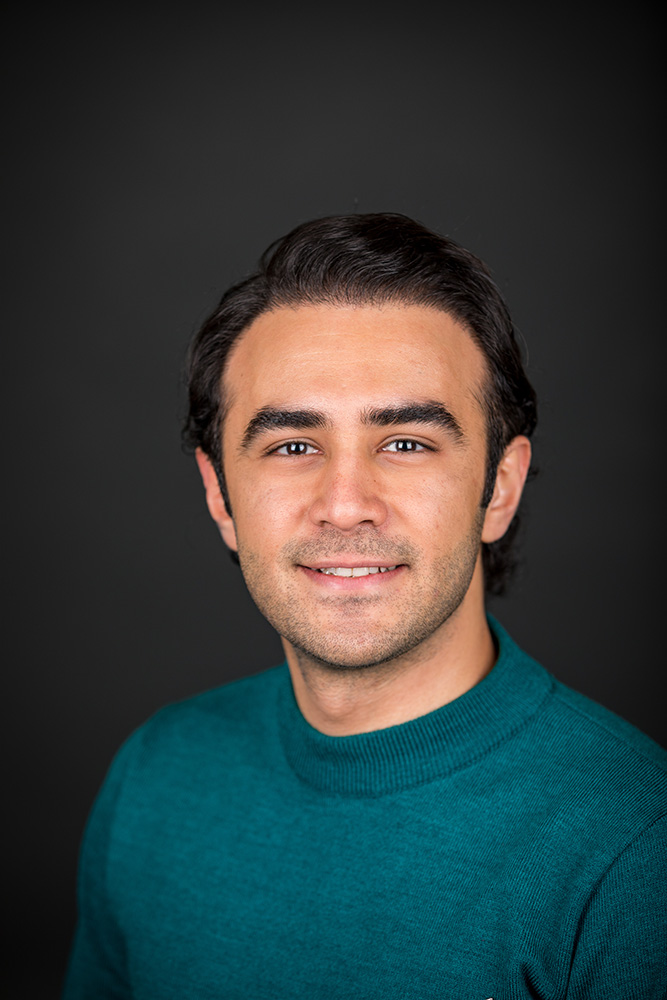
\includegraphics[width=1in,height=1.25in,clip,keepaspectratio]{Headshot.JPG}}]{Arshia Ilaty}
received the B.S. degree in computer engineering from the University of Tabriz, Iran, NV, USA, in 2021, and the M.S. degree in computer science and engineering from the University of Nevada, Reno, NV, USA, in 2023. He is currently pursuing the Ph.D. degree in computational science through a joint program at San Diego State University and the University of California, Irvine, CA, USA. His major field of study is applied machine learning and scientific computing, with a focus on healthcare and human-centered AI systems.

He has research experience spanning academia and industry. He has served as a Graduate Research Assistant at San Diego State University and the University of California, Irvine, where he develops agentic and multimodal AI systems for clinical trial optimization, pain assessment, and privacy-preserving synthetic data generation. Previously, he worked as a Software Engineer at World Mobile Inc., where he designed scalable cloud and blockchain-based systems, and as a Software Engineering Intern at Tesla, contributing to data-driven operational tooling and optimization. His research interests include multimodal machine learning, reinforcement learning, synthetic data generation, explainable AI, and high-performance computing for scientific and biomedical applications.

Mr. Ilaty is a member of the Association for Computing Machinery (ACM) and the Society for Industrial and Applied Mathematics (SIAM). He is the recipient of the Presidential Graduate Research Fellowship (UCI/SDSU), the Outstanding International Graduate Student Scholarship, and the WAAIME Scholarship. He has contributed to open-source scientific computing projects, including the libCEED and MOLE library, and has presented his work at academic conferences in applied AI.
\end{IEEEbiography}

\begin{IEEEbiography}[{\includegraphics[width=1in,height=1.25in,clip,keepaspectratio]{Shirazi.png}}]{Hossein Shirazi}
received the Ph.D. degree in electrical and computer engineering from Colorado State University, Fort Collins, CO, USA, in 2020. He is currently an Assistant Professor of Management Information Systems with the Fowler College of Business, San Diego State University, San Diego, CA, USA, where he directs the Smart Secure Systems (3S) Lab. 

His research interests lie at the intersection of cybersecurity and artificial intelligence, with specific focuses on Internet of Things (IoT) security, critical infrastructure protection, malware analysis, and adversarial machine learning. He has authored numerous publications in top-tier journals and conferences regarding the application of machine learning to enhance network security and resiliency.
\end{IEEEbiography}

\begin{IEEEbiography}[{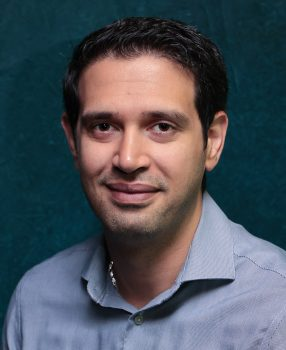
\includegraphics[width=1in,height=1.25in,clip,keepaspectratio]{Rahmani.jpg}}]{Amir M. Rahmani}
received the Ph.D. degree in computer systems from the University of Turku, Finland, in 2012, and the M.B.A. degree. He is currently a Professor with the School of Nursing and the Department of Computer Science, University of California, Irvine (UCI), Irvine, CA, USA. He is also the Founder and Director of the Health SciTech Group at UCI.

His interdisciplinary research bridges computer science and healthcare, focusing on e-health, m-health, wearable Internet of Things (IoT), bio-signal processing, and edge computing. He has led various projects on remote patient monitoring, pain assessment, and personalized healthcare systems. Dr. Rahmani has published extensively in the fields of embedded systems and healthcare IoT and serves on the editorial boards of several international journals.
\end{IEEEbiography}

\begin{IEEEbiography}[{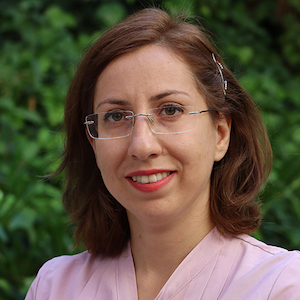
\includegraphics[width=1in,height=1.25in,clip,keepaspectratio]{homayouni.jpeg}}]{Hajar Homayouni}
received the Ph.D. degree in computer science from Colorado State University, Fort Collins, CO, USA, in 2020. She is currently an Assistant Professor with the Department of Computer Science, San Diego State University, San Diego, CA, USA, where she leads the Data Science Lab.

Her research interests include data quality, trustworthy artificial intelligence, big data management, and database systems. Her work focuses on developing methodologies to detect and repair data defects to ensure the reliability, fairness, and robustness of machine learning models. She is a member of the ACM and actively publishes in venues related to data engineering and applied AI.

\end{IEEEbiography}


\end{document}